\documentclass[a5paper, 10pt]{book}


%\usepackage[utf8]{inputenc} %Ersetzt durch LuaLaTeX
\usepackage[ngerman]{babel}
%\usepackage[T1]{fontenc}
\usepackage{fontspec}

%\usepackage{lipsum}


\onecolumn

\usepackage{amsmath}
\usepackage{amsfonts}
\usepackage{amssymb}

%für /lightning
\usepackage{wasysym}

%Identität (Relation)
\DeclareMathOperator{\id}{id}
%Realteil (komplexe Zahlen)
\DeclareMathOperator{\romanRe}{Re}
%Imaginärteil (komplexe Zahlen), Image/Bild (lineare Abbildungen)
\DeclareMathOperator{\romanIm}{Im}
%Ergebnis bei Division mit Rest
\DeclareMathOperator{\romandiv}{div}
%Rest bei Division mit Rest (ohne Leerzeichen vorher), nicht verwendet bei Kongruenz
\DeclareMathOperator{\romanmod}{mod}
%größter gemeinsamer Teiler
\DeclareMathOperator{\ggT}{ggT}
%kleinstes gemeinsames Vielfaches
\DeclareMathOperator{\kgV}{kgV}
%Ordnung (Gruppen)
\DeclareMathOperator{\ord}{ord}
%Erzeugnis (Vektorräume)
\DeclareMathOperator{\romanspan}{span}
%Kern/kernel (lineare Abbildungen)
\DeclareMathOperator{\Kern}{Kern}
%Bild (lineare Abbildungen)
\DeclareMathOperator{\Bild}{Bild}

\newcommand{\inN}{\in\mathbb{N}}
\newcommand{\inZ}{\in\mathbb{Z}}
\newcommand{\inQ}{\in\mathbb{Q}}
\newcommand{\inR}{\in\mathbb{R}}
\newcommand{\inC}{\in\mathbb{C}}
\newcommand{\NtoR}{\mathbb{N}\rightarrow\mathbb{R}}
\newcommand{\lincombine}[4]{(#1_{#3} \circlecdot #2_{#3}) \circleplus \dots \circleplus (#1_{#4} \circlecdot #2_{#4})}%Name of Scalar, Name of Vector, first index, last index
\newcommand{\entspricht}{\text{\^{=}}}
\newcommand{\matrixwithsubscript}[5]{(#1_{#2#3})_{\scriptsize\begin{array}{l}1 \leq #2 \leq #4 \\ 1\leq #3 \leq #5\end{array}}}

\newcommand{\circleplus}{\oplus}%{{\textcircled+}}
\newcommand{\circlecdot}{\otimes}%{{\textcircled.}} 
%Nullvektor
\newcommand{\boldzero}{\mathbf{0}}



\usepackage{siunitx}
%\usepackage{libertine}
\usepackage[left=1cm,right=1cm]{geometry}
\usepackage{graphics}


\usepackage{tikz}

%https://tex.stackexchange.com/questions/34452/arrow-between-parts-of-equation-in-latex
%https://tex.stackexchange.com/questions/1559/adding-a-large-brace-next-to-a-body-of-text/1570#1570
\newcommand{\tikzmark}[1]{\tikz[overlay,remember picture] \node (#1) {};}


\usepackage{pdfpages}

\usepackage{longtable}
\usepackage{xcolor}

%durchstreichen
\usepackage{cancel}

\usepackage{fancybox}

%andere Aufzählungen bei Enumerate
\usepackage{enumerate}

%links
\usepackage{hyperref}
\hypersetup{hidelinks}

%index
\usepackage{makeidx}

\usepackage{ifthen}

\makeindex



\newcommand{\keyword}[1]{\emph{#1}\index{#1@\textbf{#1}}}
\renewcommand{\keyword}[1]{\keywordUnwichitg{#1}}

\newcommand{\keywordUnwichitg}[1]{\emph{#1}\index{#1}}

\newcommand{\indexUnwichtig}[1]{\index{#1}}

\newcommand{\subkeywordNoprint}[2]{\index{#1 (#2)}\index{#2!#1}}

\newcommand{\subkeywordNoprintUnwichtig}[2]{\subkeywordNoprint{#1}{#2}}

\newcommand{\subkeyword}[2] {\ifthenelse{\equal{#2}{Halbordnung}}
				{\emph{#1}\index{#1 (#2)}\index{#2 (Mengen)!#1}\index{Mengen!#2!#1}}
				{\emph{#1}\subkeywordNoprint{#1}{#2}}} % diese Zeile wieder entfernen, falls der nachfolgende ifthenelse block benutzt wird
				%{
				%	\itthenelse{\equal{#2}{Gruppe}}{
				%		\emph{#1}\index #1 (#2)\index{#2 (Ver\-knüp\-fung\-en)!#1}\index{Ver\-knüp\-fung\-en!#2!#1}
				%	}
				%	{
				%	\emph{#1}\subkeywordNoprint{#1}{#2}}
				%	}
				%}

\newcommand{\subkeywordUnwichtig}[2]{\subkeyword{#1}{#2}}

\newcommand{\doublesubkeywordNoprint}[2]{\index{#1!#2}\index{#2!#1}}

\newcommand{\doublesubkeyword}[2]{\emph{#1}\doublesubkeywordNoprint{#1}{#2}}

\newcommand{\subsubkeywordNoprint}[3]{\index{#1 (#2, #3)}\index{#2 (#3)!#1}\index{#3!#2!#1}}

\newcommand{\subsubkeyword}[3]{\emph{#1}\subsubkeywordNoprint{#1}{#2}{#3}}

\newcommand{\indexAbbreviation}[2]{\index{#1|see{#2}}\index{#1}}

%Abbreviation/Abkürzung
\newcommand{\abbrev}[2]{\index{#1|see{#2}}\index{#1}}





%\renewcommand*{\toccontent}{\@starttoc{toc}}

\title{Mathematik für Informatiker I}
\author{Andre Johnson}

\begin{document}
	
	\maketitle
	
	\tableofcontents
	
	\chapter{Mathematische Grundlagen}
		
		\section{Aussagen}
		
			\subsection{Logische Ver\-knüp\-fung\-en (Junktoren)} \index{Junktoren}
				
				\subsubsection{Definition 1.1}
					Seine im Folgenden $A$ und $B$ Aussagen
					
					\begin{itemize}
						\item[(i)] Die \keyword{Negation} von $A$ ist die Aussage ``nicht $A$''. Wir verwenden die Schreibweise
							\begin{align}
								\neg A
							\end{align}
							Wenn $A$ wahr ist, dann ist $\neg A$ falsch. Wenn $A$ falsch ist, dann ist $\neg A$ wahr.
						\item[(ii)] Die Verbindung von $A$ und $B$ durch ``und'' heißt \keyword{Konjunktion}. Wir schreiben
							\begin{align}
								A \wedge B
							\end{align}
							$A \wedge B$ ist wahr, wenn $A$ und $B$ wahr sind, sonst falsch.
						\item[(iii)] Die Verkettung von $A$ und $B$ durch ``oder'' heißt \keyword{Disjunktion} wir schreiben
							\begin{align}
								A \vee B
							\end{align}
							$A \vee B$ ist falsch, wenn $A$ und $B$ beide falsch sind.
							
					\item[(iv)] Die Verkettung von $A$ und $B$ zu ``wenn $A$, dann $B$'' heißt \keyword{logische Folgerung} oder \keyword{Implikation}. Wir schreiben
						\begin{align}
							A \Rightarrow B
						\end{align}
						$A$ heißt \subkeyword{Voraussetzung}{Implikation}, $B$ \subkeyword{Behauptung}{Implikation} der Implikation. Die Implikation ist wahr, wenn $A$ falsch ist oder $B$ wahr ist, andernfalls ist die falsch.
					\item[(v)] Die Verkettung von $A$ und $B$ zu ``genau dann $A$, wenn $B$'' heißt \keyword{Äquivalenz}. Wir schreiben
						\begin{align}
							A \Leftrightarrow B
						\end{align}
						Die Äquivalenz ist wahr, wenn $A$ und $B$ den selben Wahrheitswert haben.
					\end{itemize}
				
					Wahrheitstafel
					\begin{longtable}{cc|cccccc}
						$A$	&	$B$ &	$\neg A$ &	$\neg B$ &	$A\wedge B$ & $A\vee B$ &	$A\Rightarrow b$ &	$A\Leftrightarrow B$\\*
						\hline
						w & w & f & f & w & w & w & w\\*
						w & f & f & w & f & w & f & f\\*
						f & w & w & f & f & w & w & f\\*
						f & f & w & w & f & f & w & w
					\end{longtable}
				
				
				\subsubsection{Definition 1.2}
					Ein logischer Ausdruck, der für beliebige Wahrheitswerte der enthaltenen Aussagen immer wahr ist, heißt \keyword{Tautologie}.
					
				
				\subsubsection{Satz 1.3}
					$A$ und $B$ seien Aussagen.\\
					Dann sind folgende Aussagen Tautologien:
					\begin{itemize}
						\item[a)] \subkeyword{De Mogan'{}sche Regeln}{Tautologie}:
							\begin{align}
								\neg\left(A\vee B\right) &\Leftrightarrow \left( \neg A \wedge \neg B \right) \\
								\neg\left(A\wedge B\right) &\Leftrightarrow \left( \neg A \vee \neg B \right)
							\end{align}
						\item[b)]
							\begin{align}
								\left( A \Rightarrow B \right) &\Leftrightarrow \left( \neg B \Rightarrow \neg A \right)
							\end{align}
					\end{itemize}
				
			\section{Mengen}\index{Mengen}
					\subsubsection{Schreibeweise:}
						$x \in M$ steht für die Aussage ``$x$ ist ein \keyword{Element} der Menge $M$''
						
						\subsubsection{Definition 1.4: Standardbezeichnungen}
							\begin{align}
								\mathbb{N} &= \left\lbrace 1, 2, 3, 4, ...\right\rbrace \text{\keyword{natürliche Zahlen}}\\
								\mathbb{N}_0 &= \left\lbrace 0, 1, 2, 3, ...\right\rbrace \text{\emph{natürliche Zahlen mit Null}\index{natürliche Zahlen!mit\ Null}}\\
								\mathbb{Z} &= \left\lbrace ..., -2, -1, 0, 1, 2, ...\right\rbrace \text{\keyword{ganze Zahlen}}\\
								\mathbb{Q} &= \left\lbrace \frac{m}{n}: m\in \mathbb{Z}, n\in \mathbb{N} \right\rbrace \text{\keyword{rationale Zahlen}}\\
								\mathbb{R}&\hspace{1em} \text{\keyword{reele Zahlen}}\\
								\emptyset&\hspace{1em} \text{\keyword{leere Menge}}
							\end{align}
							
				\subsection{Beschreibung von Mengen}\keywordUnwichitg{Beschreibung von Mengen}
					
					\begin{itemize}
						\item Durch \subkeyword{Aufzählen der Elemente}{Beschreibung von Mengen}\\
							Bsp.:
							\begin{align}
								M &= \left\lbrace 1, 2, 3\right\rbrace\\
								G &= \left\lbrace 2, 4, 6, 8, ...\right\rbrace
							\end{align}
							
						\item in \emph{beschreibender Form}\index{Beschreibung von Mengen!beschreibende Form}\\
							Bsp.:
							\begin{align}
								G &= \left\lbrace x: x \in \mathbb{N}\ \text{und}\ x\ \text{ist gerade}\right\rbrace\\
								&= \left\lbrace x \in \mathbb{N}: x\ \text{ist gerade}\right\rbrace
							\end{align}
							Allgemeine Form:
							\begin{align}
								M &= \left\lbrace x: A(x) \right\rbrace A\ \text{Aussage}
							\end{align}
							
						\item in \emph{abgekürzter beschreibender Form}\index{Beschreibung von Mengen!abgekürzte beschreibende Form}\\
							Bsp.:
							\begin{align}
								G &= \left\lbrace 2m: m\in \mathbb{N}\right\rbrace
							\end{align}
					\end{itemize}
	
			\section{Existenz- und Allquantoren}
					\subsubsection{Definition 1.5}
						Sei $M$ eine nicht-leere Menge, und für jedes $x\in M$ sei $A(x)$ eine Aussage.
						
						\begin{itemize}
							\item[(i)] Die Aussage ``Für Alle $x\in M$ gilt $A(x)$.'' bezeichnen wir mit
								\begin{align}
									\forall\ x\in M: A(x)\ \text{($\forall$ \keyword{Allquantor}\index{Quantoren!Allquantor})}
								\end{align}
						\item[(ii)] Die Aussage ``Es gibt ein $x\in M$, für das $A(x)$ gilt'' bezeichnen wir mit
							\begin{align}
								\exists\ x\in M: A(x)\ \text{($\exists$ \keyword{Existenzquantor}\index{Quantoren!Existenzquantor})}
							\end{align} 
						\item[(iii)] Die Aussage ``Es gibt genau ein $x\in M$, für das $A(x)$ gilt'' bezeichnen wir mit
							\begin{align}
								\exists!\ x\in M: A(x)
							\end{align}
						\end{itemize}
					
					\subsubsection{Lemma 1.6}
						Sei $M$ eine nicht leere Menge und für jedes $x\in M$ sei $A(x)$ eine Aussage. Dann gilt:
						\begin{align}
							\neg\left(\forall\ x\in M: A(x)\right) &\Leftrightarrow \left(\exists\ x\in M: A(x)\right)
						\end{align}
						
						
			\section{Mengenoperationen}
					\subsubsection{Definition 1.7}
					
							Seien $X$ und $Y$ Mengen
							\begin{itemize}
								\item $X$ heißt \keyword{Teilmenge} von $Y$, falls gilt
									\begin{align}
										\forall\ x\in X: x\in Y
									\end{align}
									Wir schreiben dann:
									\begin{align}
										X \subseteq Y
									\end{align}
									(\subkeyword{Inklusion}{Mengen} von $X$ in $Y$)
								\item Wenn $X$ keine Teilmenge von $Y$ ist, schreiben wir
									\begin{align}
										X \nsubseteq Y
									\end{align}
								\item $X$ heißt Teilmenge von $Y$ und $X \neq Y$: Wir schreiben dann
									\begin{align}
										X \subset Y\ &\text{oder}\ X \subsetneq Y\\
										\left( \forall\ x\in X : x\in Y \right) &\wedge \left( \exists\ y \in Y \notin X\right)
									\end{align}
								\item \subkeyword{Durchschnitt}{Mengen}
									\begin{align}
										X \cap Y &:= \left\lbrace z: z\in X \wedge z\in Y\right\rbrace
									\end{align}
								\item \subkeyword{Vereinigung}{Mengen}
									\begin{align}
										X \cup Y &:= \left\lbrace z:z \in X \vee z\in Y\right\rbrace
									\end{align}
								\item \subkeyword{Differenzmenge}{Mengen}
									\begin{align}
										X \setminus Y &:= \left\lbrace z:z\in X \wedge z\notin Y\right\rbrace
									\end{align}
								\item Falls $Y \subseteq X$, dann heißt $X\setminus Y$ das \subkeyword{Komplement}{Mengen} von $Y$ in $X$
								\item Wenn $X \cap Y = \emptyset$, dann heißen $X$ und $Y$ \subkeyword{disjunkt}{Mengen}
							\end{itemize}
					
					\subsubsection{Satz 1.8}
							Sei $M$ eine Menge und $X, Y, Z$ Teilmengen von $M$. Dann gelten
							\begin{itemize}
								\item[a)]
									\begin{align}
										M\cap \emptyset &= \emptyset\\
										X\cup M &= M\\
										X\cup \emptyset &= X\\
										X\cap M &= M
									\end{align}
								\item[b)] \subkeyword{Idempotenz}{Mengen}
									\begin{align}
										X \cup X &= X\\
										X \cap X &= X
									\end{align}
								\item[c)] \doublesubkeyword{Kommutativität}{Mengen}
									\begin{align}
										X \cap Y &= Y \cap X\\
										x \cup Y &= Y \cup X
									\end{align}
								\item[d)] \doublesubkeyword{Assoziativität}{Mengen}
									\begin{align}
										\left( X \cup Y \right) \cap Z &= X \cap \left( Y \cup Z \right)\\
										\left( X \cap Y \right) \cup Z &= X \cup \left( Y \cap Z \right)
									\end{align}
								\item[e)] 
									\begin{align}
										X \cup \left( Y \cap Z \right) &= \left( X \cup Y \right) \cap \left( X \cup Z \right)\\
										X \cap \left( Y \cup Z \right) &= \left( X \cap Y \right) \cup \left( X \cap Z \right)
									\end{align}
								\item[f)]
									\begin{align}
										M\setminus \left( X \cap Y \right) &= \left( M \setminus X \right) \cup \left( M \setminus Y \right)\\
										M\setminus \left( X \cup Y \right) &= \left( M \setminus X \right) \cap \left( M \setminus Y \right)
									\end{align}
							\end{itemize}
							Um zu beweisen, dass zwei Mengen  $A$ und $B$ gleich sind, zeigt man oft $A \subseteq B$ und $B \subseteq A$
							
					\subsubsection{Definition 1.9}
						Seien $X, Y$ Mengen.\\
						Das \subkeyword{kartesische Produkt}{Mengen} von $X$ und $Y$ ist
						\begin{align}
							X \times Y &= \left\lbrace (x, y): x\in X \wedge y\in Y \right\rbrace
						\end{align}
						$(x, y)\in X\times Y$ heißt \subkeyword{geordnetes Paar}{Mengen}.\\
						Allgemein definiert man für Mengen $X_1, X_2, ..., X_n$
						\begin{align}
							X_1 \times X_2 \times ... \times X_n &:= \left\lbrace \left(x_1, x_2, ..., x_n\right):x_i\in X_i \text{ für alle } i \in [1,n] \right\rbrace
						\end{align}
						$\left(x_1, ..., x_n\right) \in X_1 \times ...\times X_n$ heißt \subkeyword{geordnetes $n$-Tupel}{Mengen}\index{Tupel}
	
	
	\chapter{Relationen \& Funktionen}
		\section{Grundbegriffe zu Relationen}
			
			\subsubsection{Definition 2.1}
				Seien $A, B$ Mengen, $G \subseteq A \times B$\\
				Dann bezeichnet man das Tripel $(A, B, G)$ als zweistellige/binäre \keyword{Relation} zwischen $A$ und $B$. $G$ heißt \keyword{Graph} der Relation.\\
				Wenn $(a,b) \in G$, dann sagen wir, dass $a$ und $b$ in \emph{Relation zueinander stehen}, oder \emph{reliert}\indexUnwichtig{Relation!reliert sein/in Relation zueinander stehen} sind. Wir schreiben dann
				\begin{align}
					a \sim b
				\end{align}
				Falls $A = B$, heißt $(A, A, G)$ \emph{Relation auf A}\indexUnwichtig{Relation!Relation auf Menge $A$}\\
				Bemerkung: Manchmal wird $\sim$ oder $G$ als Relation bezeichnet.
				
			\subsubsection{Definition 2.2}
				Sei $A$ eine Menge, $(A, A, G)$ Relation auf $A$. Die Relation heißt
				\begin{itemize}
					\item \subkeyword{reflexiv}{Relation}, falls $a\sim a$ für jedes $a\in A$
					\item \subkeyword{symmetrisch}{Relation}, falls aus $a\sim b$ stets folgt, dass $b\sim a$
					\item \subkeyword{antisymmetrisch}{Relation}, falls aus $a\sim b \text{ und } b\sim a$ stets folgt, dass, $a = b$\footnote{$\text{antisymetrisch }\Leftrightarrow \forall\ (a,b) \in A \times B: \left((a,b)\in G \wedge (b,a) \in G\Rightarrow a=b \right)$}
					\item \subkeyword{transitiv}{Relation}, falls aus aus $a\sim b \text{ und } b\sim c$ stets folgt, dass, $a\sim c$
				\end{itemize}
			
			\subsubsection{Definition 2.3}
				Sei $(A,B,G)$ eine Relation. Setze
				\begin{align}
					G^{-1} := \left\lbrace (b,a) \in B \times A: (a,b) \in G \right\rbrace
				\end{align}
				$(B,A,G^{-1})$ heißt die zu $(A,B,G)$ \keyword{inverse Funktion}. Falls $(b,a)\in G^{-1}$, schreiben wir
				\begin{align}
					b \stackrel{-1}{\sim} a
				\end{align}
				
				
		\section{Abbildungen und Funktionen}		
			\subsubsection{Definition 2.4}
				Seien $X, Y$ Mengen\\
				Eine \keyword{Abbildung} (\keyword{Funktion} von $X$ nach $Y$) ist gegeben durch eine \subkeyword{Vorschrift}{Abbildung} $f$, die jedem Element $x\in X$ genau ein Element $y\in Y$ zuordnet. Man schreibt
				\begin{align}
					y = f(x)
				\end{align}
				Für die gesamte Abbildung schreibt man
				\begin{align}
					f: X \rightarrow Y
				\end{align}
				Für $x\in X$ schreiben wir
				\begin{align}
					x \mapsto f(x)
				\end{align}
				$X$ heißt der \subkeyword{Definitionsbereich}{Abbildung} von $f$\\
				$Y$ heißt der \subkeyword{Ziel-/Wertebereich}{Abbildung} \indexUnwichtig{Werte-/Zielberich (Abbildung)} von $f$\\
				Bemerkung: Die \keywordUnwichitg{Zuordnung} $f$ definiert eine Relation $(X, Y, G)$ durch
				\begin{align}
					(x, y) \in G :\Leftrightarrow y = f(x)
				\end{align}
				
			\subsubsection{Definition 2.5}
				Sei $f: X \rightarrow Y$ Abbildung
				\begin{itemize}
					\item Für $Z \subseteq X$ definieren wir
						\begin{align}
							f(Z) :=& \left\lbrace y \in Y: \exists x \in Z: f(x) = y \right\rbrace\\
							=&  \left\lbrace f(x): x\in Z \right\rbrace
						\end{align}
						$f(Z)$ heißt das \emph{Bild von $Z$ unter $f$}\index{Bild! von Menge $Z$ unter Funktion $f$}\\
						$f(X)$ heißt das \emph{Bild von f}\index{Bild! von Funktion $f$}
					\item Für $M\subseteq Y$ definieren wir
						\begin{align}
							f^{-1}(M) := \left\lbrace x \in X: f(x) \in M\right\rbrace
						\end{align}
						$f^{-1}$ heißt das \emph{Urbild von $M$ unter $f$}\index{Urbild von Menge $M$ unter Funktion $f$}
				\end{itemize}
			
			\subsubsection{Definition 2.6}
				\begin{figure}
					\centering
					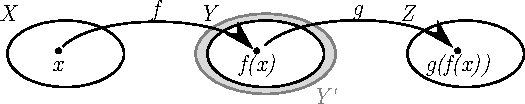
\includegraphics[width=0.7\linewidth]{img/2-6-Komposition}
					\caption{Komposition}
					\label{fig:2-6-komposition}
				\end{figure}
				Seien $f: X \rightarrow Y$ und $g: Y' \rightarrow Z$, wobei $Y \subseteq Y'$\\
				Die \keyword{Kom\-po\-si\-tion/Ver\-ket\-tung/Hin\-ter\-ei\-nan\-der\-aus\-füh\-rung} \indexUnwichtig{Ver\-ket\-tung/Kom\-po\-si\-tion/Hin\-ter\-ei\-nan\-der\-aus\-füh\-rung} \indexUnwichtig{Hin\-ter\-ei\-nan\-der\-aus\-füh\-rung/Kom\-po\-si\-tion/Ver\-ket\-tung}
				\begin{align}
					g \circ f: X \rightarrow Z
				\end{align}
				ist definiert durch
				\begin{align}
					(g\circ f)(x) = g\left( f\left(x\right)\right) \text{ für alle } x \in X
				\end{align}
				
			\subsubsection{Lemma 2.7}
				Die Komposition von Abbildungen ist \emph{assoziativ}\index{Assoziativität!Komposition}, d.~h. wenn $f: X\rightarrow Y, g: Y' \rightarrow Z$ und $h: Z' \rightarrow W$ Abbildungen sind mit $Y \subseteq Y'$ und $Z\subseteq Z'$, dann gilt
				\begin{align}
					h \circ \left( g \circ f\right) = \left( h \circ g \right) \circ f = h\circ g\circ f
				\end{align}
				
			\subsubsection{Definition 2.8}
				Eine Abbildung $f: X \rightarrow Y$ heißt
				\begin{itemize}
					\item \subkeyword{injektiv}{Abbildung}: falls für alle $a,b \in X$ gilt
						\begin{align}
							a \neq b \Rightarrow f(a) \neq f(b)
						\end{align}
					\item \subkeyword{surjektiv}{Abbildung}: falls
						\begin{align}
							f(X) = Y
						\end{align}
					\item \subkeyword{bijektiv}{Abbildung}: wenn $f$ surjektiv und injektiv ist
				\end{itemize}
		
			\subsubsection{Lemma 2.9}
				Seien $X, Y, Z$ Mengen, $f: X \rightarrow Y, g: Y \rightarrow Z$
				\begin{itemize}
					\item[1)] Wenn $f$ und $g$ surjektiv sind, dann ist auch $g\circ f$ surjektiv.
					\item[2)] Wenn $f$ und $g$ injektiv sind, dann ist auch $g\circ f$ injektiv.
					\item[3)] Wenn $f$ und $g$ bijektiv sind, dann ist auch $g\circ f$ bijektiv. 
				\end{itemize}
			
			\subsubsection{Definition 2.10}
				Sei $M$ eine Menge. Die Abbildung
				\begin{align}
					\id_X &: X \rightarrow X\\
					\id_X (x) &: x \mapsto x \text{ für alle } x\in X
				\end{align}
				heißt \emph{identische Abbildung}\index{identische Abbildung/Identität}\index{Abbildung!identische Abbildung/Identität}.
				
			\subsubsection{Satz 2.11}
				Sei $f: X \rightarrow Y$ eine Abbildung. Die folgenden Aussagen sind äquivalent:
				\begin{align}
					 (A) &\ f \text{ ist bijektiv}\\
					 (B) &\ \text{Es gibt eine Abbildung }g: Y \rightarrow X\text{, so dass }g=f=\id_X\text{ und }f=g=\id_Y
				\end{align}
				Beweis: siehe \ref{Beweis2.11}, S. \pageref{Beweis2.11}
	
		\section{Äquivalenzrelationen}
			
			\subsubsection{Definition 2.12}
				Sei $M$ eine nicht-leere Menge.\\
				Eine Relation auf $M$ heißt \keyword{Äquivalenzrelation}, wenn sie reflexiv\footnote{reflexiv: $\forall\ a\in A: a\sim a$, d.~h. $(a,a) \in G$}, symmetrisch\footnote{symmetrisch: $\forall\ a\in A:\forall\ b\in A: a\sim b\Rightarrow b\sim a$} und transitiv\footnote{transitiv: $\forall\ a\in A:\forall\ b\in A:\forall\ c\in A:\left( a\sim b\wedge b\sim c \right) \Rightarrow a\sim c$} ist. Für $x\in M$ nennt man
				\begin{align}
					[x]_\sim := [x] := \left\lbrace y\in M: x\sim y\right\rbrace
				\end{align}
				die \keyword{Äquivalenzklasse} von $x$.\\
				Die Menge aller Äquivalenzklassen bezeichnet man mit $M/\sim$
				
			\subsubsection{Definition 2.13}
				Sei $M$ eine nicht-leere Menge, $I$ eine Indexmenge.\\
				Eine \subkeyword{Partition}{Mengen} von M ist eine Menge
				\begin{align}
					\left\lbrace A_i: A_i \subseteq M, i\in I\right\rbrace
				\end{align}
				von Teilmengen von M, so dass
				\begin{itemize}
					\item[(i)]
					\begin{align}
						A_i \neq \emptyset \text{ für alle } i \in I
					\end{align}
					\item[(ii)] für $i, j\in I$ mit $i\neq j$,
						\begin{align}
							A_i \cap A_j = \emptyset
						\end{align}
					\item[(iii)]\footnote{Vereinigung aller Mengen $A_i$ mit $i\in I$}
						\begin{align}
							\bigcup_{i\in I} A_i = M
						\end{align}
				\end{itemize}
			
			\subsubsection{Satz 2.14}\label{Satz2.14}
				Sei $M$ eine nichtleere Menge
				\begin{itemize}
					\item[a)] Für jede Äquivalenzklasse auf $M$ ist $M/\sim$ eine Partition von $M$
					\item[b)] Ist $\left\lbrace A_i \subseteq M: i\in I\right\rbrace$ eine Partition von $M$, dann ist
						\begin{align}
							x\sim y:\Leftrightarrow \text{ Es gibt ein } i \in I \text{ so dass } x,y\in A_i
						\end{align}
						eine Äquivalenzrelation auf $M$. Es gilt
						\begin{align}
							M/\sim = \left\lbrace A_i:i\in I\right\rbrace
						\end{align}
				\end{itemize}
			
			\subsubsection{Definition 2.15}
				Zwei Mengen $X, Y$ heißen \subkeyword{gleichmächtig}{Mengen}, wenn es eine bijektive Abbildung $f: X\rightarrow Y$ gibt.\\
				Eine Menge $M$ heißt \subkeyword{endlich}{Mengen}, wenn sie gleichmächtig ist zu einer Menge der Form $\lbrace 1, 2, 3, ..., n\rbrace$ für $n\in \mathbb{N}$.
				$n\in N$ heißt \subkeyword{Mächtigkeit}{Mengen} von $M$. Wir schreiben
				\begin{align}
					\left|M\right| = n
				\end{align}
				Ist $M$ nicht endlich, so schreibt man
				\begin{align}
					\left| M \right| = \infty
				\end{align}
			
		\section{Ordnungsrelation}
			
			\subsubsection{Definition 2.16}
				\begin{itemize}
					\item[a)] Eine \subkeyword{Halbordnung}{Mengen} auf eine Menge $M$ ist eine reflexive, antisymmetrische\footnote{antisymmetrisch: $\forall\ (a,b) \in M \times M: a\sim b \wedge b\sim a \Rightarrow a = b$} und transitive Relation auf $M$.
					\item[b)] Eine \subkeyword{totale/binäre Ordnung}{Mengen}\indexUnwichtig{binäre/totale Ordnung (Mengen)} auf $M$ ist eine Halbordnung auf $M$, so dass für alle $x,y\in M$ gilt $x\sim y$ oder $y\sim x$
				\end{itemize}
			
				\paragraph{Notation:}
					Für Halbordnungen schreiben wir für $x\sim y$ gerne
					\begin{align}
						x \preccurlyeq y
					\end{align}
					
				\paragraph{Bemerkung:}
					Halbordnungen können durch \emph{Hasse-Diagramme}\index{Mengen!Halbordnung!Hasse-Daigramm}\index{Halbordnung (Mengen)!Hasse-Diagramm} dargestellt werden. Man verbindet $a$ und $b$ durch eine Kante, wenn $a \preccurlyeq b$ und es kein drittes Element $c$ ($c\neq a, c\neq b$) gibt, so dass $a \preccurlyeq c \preccurlyeq b$. Im Hasse-Diagramm steht $b$ über $a$.\\
					Bsp.: $\lbrace 1,2,3\rbrace$ mit $\leq$ Relation:
					
					\begin{center}
					\begin{tikzpicture}
						\node at (0,0) {$3$};
						\draw (0, -0.2) -- (0, -0.5);
						\node at (0, -0.7) {$2$};
						\draw (0, -0.9) -- (0,-1.2);
						\node at (0, -1.4) {$1$};
					\end{tikzpicture}
					\end{center}
				
				
			\subsubsection{Definition 2.17}
				Sei $A$ eine halbgeordnete Menge, $T \subseteq A$ Teilmenge.
				\begin{itemize}
					\item[\textcircled 1] Ein Element $m\in T$ heißt \subkeyword{minimal}{Halbordnung} in $T$, wenn es kein $t \in T$ mit $t \neq m$ und $t \preccurlyeq m$. (entsprechend ``\subkeyword{maximal}{Halbordnung}'')
					\item[\textcircled 2] Wenn $m\in T$ und $m \preccurlyeq t$ für alle $t\in T$, dann heißt $m$ \subkeyword{Minimum}{Halbordnung} von $T$. (entsprechend ``\subkeyword{Maximum}{Halbordnung}'')
					\item[\textcircled 3] Wenn $s \in A$ und $s \preccurlyeq t$ für alle $t \in T$, dann heißt $s$ \subkeyword{untere Schranke}{Halbordnung} für $T$ in $A$. (entsprechend ``\subkeyword{obere Schranke}{Halbordnung}'')
				\end{itemize}
			%TODO Beispiel
			\paragraph{Beispiel} Betrachte Menge $A = \lbrace a,b,c,d,e,f,g\rbrace$ mit Halbordnung gegeben durch Hasse-Diagramm. Betrachte Teilmenge $T = \lbrace a,b,c\rbrace$
			\paragraph{Bemerkung}
			Die ``größte'' untere Schranke $e$ (d.~h. $e$ ist untere Schranke und für jede untere Schranke $s$ gilt $s\preccurlyeq e$) heißt \subkeyword{Infimum}{Halbordnung} von $T$ in $A$.\\
			Die ``kleinste'' obere Schranke heißt \subkeyword{Supremum}{Halbordnung}.
			
	\chapter{Zahlenbereiche}
		\section{Natürliche Zahlen: Definition}
			
			\index{natürliche Zahlen}
			\subsubsection{Definition 3.1: Peano-Axiome}
				
				\begin{itemize}
					\item[\textcircled 1] $1$ ist eine natürliche Zahl.
					\item[\textcircled 2] Jede natürliche Zahl hat genau einen von $1$ verschiedenen Nachfolger $n^+$, der eine natürliche Zahl ist (gemeint ist $n+1$).
					\item[\textcircled 3] Verschiedene natürliche Zahlen haben verschiedene Nachfolger.
					\item[\textcircled 4] Ist $M \subseteq \mathbb{N}$ mit $1\in M$ und der Eigenschaft, dass für alle $n\in M$ auch $n^+ \in M$ folgt, so gilt $M = \mathbb{N}$ 
				\end{itemize}
			
			\subsection{Notation: Produkt- und Summenschreibweise}\index{Produktschreibweise}\index{Summenschreibweise}
				
				Seien $k,n\in \mathbb{N}$ und $a_j \in \mathbb{C}$ oder $\mathbb{R}$. Wir schreiben:
				
				\begin{align}
					\sum_{j=k}^{n} a_j := \left\lbrace 
						\parbox{0.3\linewidth}{
							$0  \text{ falls } n < k$\\
							$a_k  \text{ falls } n = k$\\
							$\sum_{j=k}^{n-1}  \text{ falls } n > k$
						}\right.\\
					\prod_{j=k}^{n} a_j := \left\lbrace 
					\parbox{0.3\linewidth}{
						$1  \text{ falls } n < k$\\
						$a_k  \text{ falls } n = k$\\
						$\prod_{j=k}^{n-1}  \text{ falls } n > k$
					}\right.
				\end{align}
			
		\section{Vollständige Induktion}\index{Vollständige Induktion}\index{Induktion}
		
			\paragraph{Idee} Für $n\in \mathbb{N}$ sei $A(n)$ eine Aussage über $n$. Ist die Aussage $A(1)$ wahr (``\subkeyword{Induktionsanfang}{Induktion}'') und folgt für jedes $n\in \mathbb{N}$ die Aussage $A(n+1)$ (``\subkeyword{Induktionsschritt}{Induktion}''), dann ist $A(n)$ wahr für alle $n\in\mathbb{N}$. %TODO Anführungsstriche reparieren
			\paragraph{Beweisskizze} Sei
				\begin{align}
					M := \{ n\in \mathbb{N}: A(n) \text{ wahr} \}
				\end{align}
				Dann
				\begin{align}
					1\in M \text{ (Induktionsanfang)}
				\end{align}
				Falls $n\in M$, dann gilt
				\begin{align}
					(n+1)\in M \text{ (Induktionsschritt)}
				\end{align}
				Nach Peano {\textcircled 4} $M=\mathbb{N}$\hspace{2em} {$\Box$}
				
			\subsubsection{Lemma 3.2}
				Für alle $n\in \mathbb{N}$ gilt
					\begin{align}
						1+ \dots +n := \sum_{j=1}^{n} j = \frac{n(n+1)}{2}
					\end{align}
			
			\subsubsection{Definition 3.3}\index{Potenz}
				Für $n\in \mathbb{N}_0$ und $a \in \mathbb{C}$ setzt man
				\begin{align}
					a^n := \prod_{j=1}^n a\\
					\text{Insbesondere: } a^0 = 1 
				\end{align}
				Für $a\neq 0$ und $n \in \mathbb{Z}$ mit $n < 0$ setzt man
				\begin{align}
					a^n := (a^{-1})^{-n}, a^{-1} = \frac{1}{a} 
				\end{align}
				
			\subsubsection{Lemma 3.4}
				Sei $x\in \mathbb{R}, x \neq 1$. Dann gilt für alle $n\in \mathbb{N}_0$
				\begin{align}
					1 + x + \dots + x^n = \sum_{j=0}^{n} x^j = \frac{1-x^{n-1}}{1-x}
				\end{align}
				
		\section{Rekursive Abbildungen}
			
			\subsubsection{Beispiel:}\indexUnwichtig{Summe, rekursiv}\indexUnwichtig{Produkt, rekursiv}
				\begin{align}
					\sum_{j=n}^{n} a_j := a_n &, \sum_{j=n}^N := \sum_{j=n}^{N-1} a_j + a_N \text{ für } N > n\\
					\prod_{j=n}^{n} a_j := a_n &, \prod_{j=n}^N := \left(\prod_{j=n}^{N-1} a_j\right) \cdot a_N \text{ für } N > n
				\end{align}
				
			\subsubsection{Definition 3.5}\index{Fakultät}
				Für $n\in \mathbb{N}_0$ definieren wir
				\begin{align}
					n! := \left\lbrace 
					\parbox{0.3\linewidth}{
						$1  \text{ falls } n = 0$\\
						$(n-1)!\cdot n  \text{ falls } n \geq 1$
					}\right.
				\end{align}
				D.~h.: $n! = 1 \cdot 2 \cdot \dots \cdot n$ für $n \geq 1$
				
			\subsubsection{Lemma 3.6}
				Für alle $n\in \mathbb{N}$ mit $n \geq 4$ gilt
				\begin{align}
					n! > 2^n = \underbrace{2\cdot 2 \cdot \dots \cdot 2}_{n\text{ Faktoren}}
				\end{align}
				
			\subsubsection{Beispiel: Die Fibonacci-Zahlen}\indexUnwichtig{Fibonacci-Zahlen}
				\begin{align}
					F(n)&, n\in \mathbb{N} \text{ sind rekursiv definiert:}\\
					F(1) &:= 1, F(2) := 1, F(n+1) := F(n) + F(n-1), n \geq 2\\
					\text{Also: } F(3) &= F(2) + F(1) = 1+1 = 2\\
					F(4) &= F(3) + F(2) = 3\\
					F(5) &= 5
				\end{align}
				
			\subsubsection{Lemma 3.7}
				Für alle $n \in \mathbb{N}$ gilt $F(n) < 2^n$
				
		\section{Ganze, rationale und reelle Zahlen}
			Wir werden die ganzen Zahlen
			\begin{align}
				\mathbb{Z} = \lbrace \dots, -2, -1, 0, 1, 2, \dots \rbrace,
			\end{align}
			die rationalen Zahlen
			\begin{align}
				\mathbb{Q} = \left\lbrace \frac{m}{n}: m\in \mathbb{Z}, n \in \mathbb{N}\right\rbrace
			\end{align}
			und die reellen Zahlen $\mathbb{R}$ nicht mathematisch sauber einführen, sondern ``naiv'' verwenden. Es gilt
			\begin{align}
				\mathbb{N} \subset \mathbb{Z} \subset \mathbb{Q} \subset \mathbb{R}
			\end{align}
			und wir verwenden die bekannte Totalordnung auf diese Mengen
			\begin{align}
				\text{Wichtig: } a \geq b \Leftrightarrow -b \geq -a
			\end{align}
			Für rationale Zahlen (``Brüche'') $\frac{a}{b}$ und $\frac{c}{d} \in \mathbb{Q}$ definiert man
			\begin{align}
				\frac{a}{b} + \frac{c}{d} = \frac{ad + cb}{bd}\\
				\text{Bsp.:  } \frac{2}{3} + \frac{1}{4} = \frac{11}{12} = \frac{8+3}{12}
			\end{align}
			und
			\begin{align}
				\frac{a}{b} \cdot \frac{c}{d} = \frac{a\cdot c}{b \cdot d}\\
				\text{Bsp.:} \frac{2}{3} \cdot \frac{1}{4} = \frac{2}{12} = \frac{1}{6}
			\end{align}
			Die reellen Zahlen kann man sich vorstellen, als die Menge aller Dezimaldarstellungen. Der Übergang von $\mathbb{Q}$ zu $\mathbb{R}$ ``füllt'' man die ``Löcher'' im Zahlenstrahl.
			
		\section{Komplexe Zahlen}
		
			Wir starten bei $\mathbb{R}$ und fügen das Element $i$\subkeywordNoprint{i@$i$}{komplexe Zahlen} dazu mit der Eigenschaft
			\begin{align}
				i^2 = -1
			\end{align}
			$i$ heißt auch \subkeyword{imaginäre Zahl}{komplexe Zahlen}.
			
			\subsubsection{Definition 3.8}
				Wir definieren die Menge $\mathbb{C}$ der \emph{komplexen Zahlen}\index{komplexe Zahlen}
				\begin{align}
					\mathbb{C} = \{a + bi: a, b \inR\}
				\end{align}
				wobei
				\begin{align}
					a + bi = a' + b'i :\Leftrightarrow a = a' \wedge b = b'
				\end{align}
				Für eine komplexe Zahl $z = a + bi$ mit $a,b\inR$ nennt man
				\begin{align}
					a = \romanRe(z)& \text{ den \subkeyword{Realteil}{komplexe Zahlen} und}\\
					b = \romanIm(z)& \text{ den \subkeyword{Imaginärteil}{komplexe Zahlen}}
				\end{align} 
				\paragraph{Bemerkung} $\romanRe(z)$ und $\romanIm(z)$ sind reelle Zahlen.
				\paragraph{Definition 3.8 (fortgesetzt)}~\\
				Für komplexe Zahlen $a + bi, c+ di$ mit $a,b,c,d\inR$ definiert man
				\begin{align}
					(a + bi) + (c + di) &= (a+c) + (b+d)i \hspace{3em} \text{und}\\
					(a + bi) \cdot (c + di) &= (ac - bd) + (ad + bc)i
				\end{align}
				\index{komplexe Zahlen!Additon}\index{komplexe Zahlen!Multiplikation}Addition von komplexen Zahlen entspricht der Addition von Vektoren.
				
			\subsubsection{Definition.3.9}
				Für $z = a + bi \inC$ mit $a,b\inR$ heißt
				\begin{itemize}
					\item $\left| z\right| := \sqrt{a^2 + b^2} \inR$ der \subkeyword{Betrag}{komplexe Zahlen} von $z$
					\item $\overline{z} := a-bi \inC$ die \subkeyword{konjugent-komplexe Zahl}{komplexe Zahlen}
				\end{itemize}
			
			\subsubsection{Lemma 3.10}
				Seien $z, w \inC$. Dann gilt:
				\begin{itemize}
					\item[(i)] $\overline{\overline{z}} = z$
					\item[(ii)] $\overline{z+w} = \overline{z} + \overline{w}$
					\item[(iii)] $\overline{z\cdot w} = \overline{z} \cdot \overline{w}$
					\item[(iv)] $\left| z\cdot w\right| = \left| z\right| \cdot \left| w \right|$
					\item[(v)] $\left| \overline{z}\right| = \left| z\right|$
				\end{itemize}
			
	\chapter{Folgen und Grenzwerte}
			
			\subsubsection{Definition 4.1}
				Eine (reelle) \emph{Folge}\index{Folgen} ist eine Abbildung $a: \mathbb{N} \rightarrow \mathbb{R}$. Wir schreiben $a_n = a(n)$.\\
				$a_n$ heißen \subkeyword{Glieder}{Folgen} der Folge $a$.
			
			\subsubsection{Definition 4.2: Beschränktheit}\subkeywordNoprint{Beschränktheit}{Folgen}
				Eine Folge $a: \mathbb{N} \rightarrow \mathbb{R}$ heißt \emph{beschränkt}, falls es ein $L\inR$ gibt, so dass $\left| a_n \right| \leq L$ für alle $n \inN$. Das heißt
				\begin{align}
					\exists L \inR: \forall n \inN. \left|a_n \right| \leq L
				\end{align}
				
		\section{Konvergenz}\subkeywordNoprint{Konvergenz}{Folgen}
			
			\subsubsection{Definition 4.3}
				Sei $a: \NtoR$ eine Folge, und $a_* \inR$. Die Folge $a$ konvergiert gegen $a_*$, falls gilt
				\begin{align}
					\forall \varepsilon > 0\ \exists N_0 \inN\ \forall n \geq N_0: \left| a_n - a_*\right| < \varepsilon
				\end{align}
				Wir schreiben dann $\lim\limits_{n\rightarrow \infty} a_n = a_*$ oder $a_n \rightarrow a_*$.\\
				$a_*$ heißt dann \subkeyword{Grenzwert}{Folgen} der Folge $a$\\
				$a$ heißt \subkeywordUnwichtig{konvergent}{Folgen}\\
				Falls eine Folge nicht konvergent ist, heißt sie \subkeywordUnwichtig{divergent}{Folgen}\index{Folgen!Divergenz}
				\paragraph{Bemerkung:}
					\begin{itemize}
						\item Eine Folge, die gegen 0 konvergiert heißt \subkeyword{Nullfolge}{Folgen}
						\item Eine Folge $a$ ist genau dann eine Nullfolge, wenn $|a|:\NtoR, |a|_n := |a_n|$ eine Nullfolge ist
						\item Eine Folge $a: \NtoR$ konvergiert gegen $a_* \inR$ genau dann, wenn $(a-a_*): \NtoR, (a-a_*)_n := a_n - a_*$ eine Nullfolge ist
						\item Eine Menge der Form $(-\varepsilon+x, x+\varepsilon), \varepsilon > 0$ heißt (offene) Umgebung von $x$. \subkeywordNoprintUnwichtig{Umgebung von $x$}{Folgen}\\
						Konvergiert eine Folge $a$ gegen $a_*$, dann liegen in jeder Umgebung von $a_*$ alle bis auf endlich viele Folgenglieder.
					\end{itemize}
					%TODO Beispiele
					
			\subsubsection{Satz 4.4}
				Sei $a: \NtoR$ eine konvergente Folge. Dann ist der Grenzwert $a_*$ eindeutig bestimmt.
				
			\subsubsection{Satz 4.5}
				Jede konvergente Folge ist beschränkt.
				
			\subsubsection{Satz 4.6}
				Seien $a,b: \NtoR$ konvergente Folgen $\lim\limits_{n\to\infty}a_n = a_*, \lim\limits_{n\to\infty}b_n = b_*$. Dann gilt:
				\begin{enumerate}
					\item $\lim\limits_{n\to\infty}(\alpha a_n + \beta b_n) = \alpha a_* + \beta b_*, \alpha, \beta \inR$
					\item $\lim\limits_{n\to\infty}(a_n\cdot b_n = a_* + b_*)$
					\item $\lim\limits_{n\to\infty}|a_n| = |a_*|$
				\end{enumerate}
			
			\subsubsection{Satz 4.7: Sandwich-Theorem}
				Seien $a,b,c: \NtoR$ Folgen und $N_0 \inN$ so dass
				\begin{align}
					\lim\limits_{n\to\infty} a_n = g &= \lim\limits_{n\to\infty} c_n \hspace{3em}\text{und}\\
					a_n \leq b_n &\leq c_n \text{ für alle } n \inN
				\end{align}
				Dann konvergiert auch $b$ und es gilt $\lim\limits_{n\to\infty} b_n = g$
				\paragraph{Bemerkung}
					Wenn es ein $N_0\inN$ gibt, so dass eine Aussage für für alle $n\geq N_0$ gilt, dann sagt man, die Aussage gilt für fast alle $n\inN$.\subkeywordNoprintUnwichtig{die Aussage gilt für fast alle $n\inN$}{Folgen} (D.~h. für alle $n\inN$ bis auf endlich viele)
			
			\subsubsection{Korollar 4.8}
				Ist $a: \NtoR$ beschränkt und $b:\NtoR$ eine Nullfolge, so gilt $\lim\limits_{n\to\infty} (a_n\cdot b_n) = 0$.
				
			\subsubsection{Lemma 4.9}
				Seien $a,b: \NtoR$ konvergente Folgen mit $a_n \leq b_n$ für fast alle $n\inN$. Dann gilt
				\begin{align}
					\lim\limits_{n\to\infty} a_n \leq \lim\limits_{n\to\infty} b_n
				\end{align}
				
			\subsubsection{Definition 4.10}
				Sei $f: \mathbb{N}\to\mathbb{N}$ eine wachsende Funktion:
				\begin{align}
					f(1) < f(2) < f(3) < \dots <
				\end{align}
				Sei $a: \NtoR$ eine reelle Folge: Dann heißt
				\begin{align}
					a_f: \NtoR, a_f(n) = a_{f(n)}
				\end{align}
				\subkeyword{Teilfolge}{Folgen} von $a$.
				\paragraph{Beispiel} 
				\begin{align}
					f: \mathbb{N}\to\mathbb{N}, f(n) = 2n\\
					a_f: a_2, a_4, a_6, \dots
				\end{align}
				\paragraph{Bemerkung} Wenn $a$ konvergiert, dann konvergieren auch alle Teilfolgen gegen den selben Grenzwert.\\
				Eine Folge kann konvergente Teilfolgen haben, ohne selbst zu konvergieren.\\(Bsp.: $a:\mathbb{N}\to\mathbb{N}, a_n = (-1^n)$)
				
		\section{Monotone Folgen}
			
			\subsubsection{Definition 4.11}\subkeywordNoprint{Monotonie}{Folgen}
				Eine Folge $a: \NtoR$ heißt
				\begin{itemize}
					\item \subkeyword{monoton wachsend}{Folgen}, falls $a_{n+1} \geq a_{n}$ für alle $n\inN$
					\item \subkeyword{monoton fallend}{Folgen}, falls $a_{n+1} \leq a_{n}$ für alle $n\inN$
					\item \subkeyword{monoton}{Folgen}, wenn die monoton wachsend oder monoton fallend ist.
				\end{itemize}
				\paragraph{Beispiel} $a_n = \frac{1}{n}$ monoton fallend, $b_n = n$ monoton wachsend
				
			\subsubsection{Satz 4.12 Monotoniekriterien}
				Sei $a \NtoR$ eine monotone und beschränkte Folge. Dann konvergiert $a$, d.~h. es gibt $a_*\inR$ so dass $\lim\limits_{n\to\infty} a_n = a_*$
				
		\section{Uneigentliche Konvergenz}
			
			\subsubsection{Definition 4.13}
				\subkeywordNoprint{uneigentlich konvergent gegen $\pm\infty$@(uneigentlich) konvergent gegen $\pm\infty$}{Folgen}\subkeywordNoprintUnwichtig{konvergent gegen $\pm\infty$}{Folgen}
				Eine Folge $a: \NtoR$ heißt \emph{(uneigentlich) konvergent gegen $\infty$}, wenn gilt
				\begin{itemize}
					\item $a_n > 0$ für fast alle $n\inN$
					\item $\frac{1}{a_n} \to 0$
				\end{itemize}
				Schreibweise:
				\begin{align}
					\lim\limits_{n\to\infty} a_n = \infty
				\end{align}
				\emph{(uneigentlich) konvergent gegen $-\infty$}, falls gilt
				\begin{itemize}
					\item $a_n < 0$ für fast alle $n\inN$
					\item $\frac{1}{a_n} \to 0$
				\end{itemize}
				Schreibweise:
				\begin{align}
				\lim\limits_{n\to\infty} a_n = -\infty
				\end{align}
				\paragraph{Beispiel}
				\begin{itemize}
					\item $a_n = n$: uneigentlich konvergent gegen $\infty$
					\item $b_n = -n$: uneigentlich konvergent gegen $-\infty$
					\item $c_n = (-1)^n \cdot n$: nicht uneigentlich konvergent
				\end{itemize}
		
			\subsubsection{Satz 4.14}
				Sei $a:\NtoR$ monoton und nicht beschränkt. Dann ist $a$ uneigentlich konvergent.
		
		\section{Landau-Symbole}
		
			\subsubsection{Definition 4.15}
				Sei $r: \NtoR$ Referenzfolge
				\begin{align}
					\mathcal{O}(r)&\ := \left\lbrace a:\NtoR: \exists c > 0 \text{ so dass } |a_n| \leq c\cdot |r_n| \text{ für fast alle } n\inN\right\rbrace\\
					o(r)&\ := \left\lbrace a:\NtoR: \text{ Für jedes } c > 0 \text{ gilt } |a_n| \leq c\cdot |r_n| \text{ für fast alle } n\inN\right\rbrace\\
					\Theta(r)&\ := \left\lbrace a:\NtoR: a \in \mathcal{O}(r) \text{ und } r \in \mathcal{O}(a)\right\rbrace
				\end{align}
				
			\subsubsection{Lemma 4.16}
				\begin{align}
					a \in o(r) \implies a \in \mathcal{O}(r)
				\end{align}
				Es gilt:
				\begin{align}
					\dots \subseteq \mathcal{O}\left(\frac{1}{n^2}\right) \subseteq \mathcal{O} \left(\frac{1}{n}\right) \subseteq \mathcal{O}(1) \subseteq \mathcal{O}\left(n\right) \subseteq \mathcal{O} \left(n^2\right) \subseteq \dots
				\end{align}
				
			\subsubsection{Satz 4.17}
				Sei $r: \NtoR\backslash \{0\}$. Dann gilt
				\begin{align}
				\intertext{a)}
					\mathcal{O}(r) &= \left\lbrace a: \NtoR: \underbrace{\left|\frac{a}{r}\right|}_{\text{Folge mit Gliedern } \frac{a_n}{r_n}} \text{ beschränkt} \right\rbrace\\
					\intertext{b)}
					o(r) &= \left\lbrace a: \NtoR : \lim\limits_{n\to\infty}\left|\frac{a_n}{r_n}\right|= 0\right\rbrace
				\end{align}
				
			\subsubsection{Satz 4.18 L'Hospital'sche Regel}\subkeywordNoprint{L'Hospital'sche Regel}{Folgen}
				Folgen $a: \NtoR$ und $r: \NtoR$ seinen gegeben durch differenzierbare Funktionen, d.~h. $a_n = \tilde{a}, r_n = \tilde{r}$ mit diff.baren Funktionen $\tilde{a}, \tilde{r}$.\\
				Falls gilt
				\begin{itemize}
					\item $\lim\limits_{n\to\infty} \left|r_n\right| = 0$
					\item $r'(n) \neq 0$ für fast alle $n\inN$
					\item $\lim\limits_{n\to\infty} \frac{a'(n)}{r'(n)}$ existiert eigentlich oder uneigentlich
				\end{itemize}
			Dann gilt
			\begin{align}
				\lim\limits_{n\to\infty} \frac{a'(n)}{r'(n)} = \lim\limits_{n\to\infty} \frac{a(n)}{r(n)}
			\end{align}
			
	\chapter{Der Ring $\mathbb{Z}$}
		
		\section{Gruppen}
			
			\subsubsection{Definition 5.1}
			
				Sei $M$ eine Menge. Eine \emph{Verknüpfung}\index{Ver\-knüp\-fung\-en}\index{Abbildung!Ver\-knüp\-fung\-en}\index{Mengen!Ver\-knüp\-fung\-en} $\circ$ auf M ist eine Abbildung
				\begin{align}
					\circ: M\times M \to M
				\end{align}
				Die Verknüpfung heißt \emph{assoziativ}\doublesubkeywordNoprint{Assoziativität}{Ver\-knüp\-fung\-en}, falls
				\begin{align}
					(x\circ y)\circ z = x \circ (y \circ z) \text{ für alle } x, y, z \in M
				\end{align}
				Sie heißt \emph{kommutativ}\doublesubkeywordNoprint{Kommutativität}{Ver\-knüp\-fung\-en}, falls
				\begin{align}
					x \circ y = y \circ x \text{ für alle } x, y \in M
				\end{align}
				
			\subsubsection{Definition 5.2}
				\begin{itemize}
					\item[a)] Eine Menge $H$ mit einer assoziativen Verknüpfung $\circ$ heißt \subkeyword{Halbgruppe}{Ver\-knüp\-fung\-en} $(H,\circ)$.
					\item[b)] Eine Halbgruppe $(H,\circ)$ heißt \subkeyword{Monoid}{Ver\-knüp\-fung\-en}, wenn es ein $e\in M$ gibt mit
					\begin{align}
						e \circ m = m \circ e = m \text{ für alle } m \in M
					\end{align}
					Dann heißt $e$ \subkeyword{neutrales Element}{Ver\-knüp\-fung\-en} des Monoid.
					\item[c)] Ein Monoid $(G, \circ)$ heißt \subkeyword{Gruppe}{Ver\-knüp\-fung\-en}, falls gilt: Zu jedem $x \in G$ gibt es ein $x'\in G$ so dass
					\begin{align}
						x \circ x' = x' \circ x = e
					\end{align}
					Dann heißt $x'$ \emph{``zu $x$ }\subkeyword{inverses Element}{Ver\-knüp\-fung\-en}\emph{''}.
					\item[d)] Eine Gruppe mit kommutativer Verknüpfung heißt \emph{kommutative} oder \emph{abelsche Gruppe}.\subkeywordNoprintUnwichtig{kommutative/abelsche Gruppe}{Ver\-knüp\-fung\-en}\subkeywordNoprint{abelsche/kommutative Gruppe}{Ver\-knüp\-fung\-en}
				\end{itemize}
			
				\paragraph{Beispiele}
					\begin{itemize}
						\item ``$+$'' ist eine assoziative und kommutative Verknüpfung auf $\mathbb{N}, \mathbb{Z}, \mathbb{Q}, \mathbb{R}$.
						\item $(\mathbb{N}, +)$ ist kein Monoid, da $0 \notin\mathbb{N}$.
						\item $(\mathbb{Z}, +)$ ist abelsche Gruppe, $0$ ist neutrales Element.
						\item ``$\cdot$'' ist assoziative Verknüpfung auf $\mathbb{N}, \mathbb{Z}, \mathbb{Q}, \mathbb{R}$.
						\item $(\mathbb{Q},\times)$ ist Monoid aber keine Gruppe, da $0$ kein inverses Element hat.
						\item $(\mathbb{Q}\backslash\{0\}, \cdot)$ ist abelsche Gruppe.
					\end{itemize}
			
			\subsubsection{Lemma 5.3}
				Ein Monoid hat genau ein neutrales Element.
				\paragraph{Beweis} Angenommen $e$ und $f$ sind neutrale Elemente. $e = e\circ f = f\hspace{3em} \square$
				
			\subsubsection{Lemma 5.4}
				Ist $(G,\circ)$ eine Gruppe und $x \in G$. Dann gibt es genau ein inverses Element $y\in G$ zu $x$.
				\paragraph{Beweis} Seien $y,z\in G$ inverse Elemente zu $x$. Dann gilt\\
				$y = y\circ e = y \circ (x \circ z) = (y\circ x) \circ z = e \circ z = z \hspace{3em} \square$
				
			\subsubsection{Lemma 5.5}
				Sei $(G, \circ)$ eine Gruppe, $x,y\in G$. Seien $x'$ das inverse Element zu $x$, und $y'$ das inverse Element zu $y$. Dann ist $(x\circ y)' := y' \circ x'$ das inverse Element zu $x \circ y$.
				\paragraph{Beweis} $(x\circ y)\circ(y'\circ x') = (x\circ (y\circ y')) \circ x' = (x \circ e) \circ x' = x \circ x' = e \hspace{3em} \square$
				
		\section{Ringe und Körper}
			
			\subsubsection{Definition 5.6}
				Sei $R$ eine Menge mit zwei Ver\-knüp\-fung\-en
				\begin{itemize}
					\item[$\circleplus$] \subkeyword{Addition}{Ver\-knüp\-fung\-en}
					\item[$\circlecdot$] \subkeyword{Multiplikation}{Ver\-knüp\-fung\-en}
				\end{itemize}
			so dass gilt
			\begin{itemize}
				\item[1)] $(R, \circleplus)$ ist abelsche Gruppe mit neutralem Element  $0\in R$
				\item[2)] $(R, \circlecdot)$ ist Halbgruppe:
				\item[3)] \subkeyword{Distributivität}{Ver\-knüp\-fung\-en}:
					\begin{align}
					x \circlecdot (y \circleplus z) &= (x\circlecdot y)\circleplus(x\circlecdot z)\text{ und}\\
					(y \circleplus z) \circlecdot x &= (y \circlecdot x) \circleplus (z \circlecdot x) \text{ für alle } x,y,z\in R
					\end{align}
			\end{itemize}
			Dann ist $(R, \circleplus, \circlecdot)$ ein \subkeyword{Ring}{Ver\-knüp\-fung\-en}.
			\begin{itemize}
				\item $(R, \circleplus, \circlecdot)$ heißt \subkeyword{Ring mit Eins}{Ver\-knüp\-fung\-en}, falls $(R, \circlecdot)$ ein Monoid ist, dessen neutrales Element $1\in R$ ungleich dem neutralen Element $0$ er Addition ist.
				\item Der Ring $(R, \circleplus, \circlecdot)$ heißt \emph{kommutativ}\index{Kommutativität!Ring (Ver\-knüp\-fung\-en)}\index{Ver\-knüp\-fung\-en!Ring!Kommutativität}\index{Ver\-knüp\-fung\-en!Kommutativität (Ring)}, falls $\circlecdot$ kommutativ ist.
				\item Ein kommutativer Ring mit Eins $(R, \circleplus, \circlecdot)$ heißt \subkeyword{Körper}{Ver\-knüp\-fung\-en}, wenn jedes Element $x\neq 0$ ein multiplikatives Inverses hat.
			\end{itemize}
			\paragraph{Beispiele}
				\begin{itemize}
					\item $(\mathbb{Z}, +, \cdot)$ kommutativer Ring mit Eins
					\item $(2\mathbb{Z}, +, \cdot)$ kommutativer Ring ohne Eins
					\item $(\mathbb{R}, +, \cdot)$ Körper
					\item $(\mathbb{Q}, +, \cdot)$ Körper
					\item Auf $M = \{0,1\}$ definiere
						\begin{tabular}{ccc}
							\begin{tabular}{c|cc}
								$\circleplus$ & $0$ & $1$\\
								\hline
								$0$ & $0$ & $1$\\
								$1$ & $1$ & $0$
							\end{tabular}
							&
							\begin{tabular}{c|cc}
								$\circlecdot$ & $0$ & $1$\\
								\hline
								$0$ & $0$ & $0$\\
								$1$ & $0$ & $1$
							\end{tabular}
							&
							Körper
						\end{tabular}
				\end{itemize}
			
			
			\subsubsection{Lemma 5.7}
				Sei $(R,\circleplus,\circlecdot)$ ein Ring, $0$ das neutrale Element bzgl. der Addition. Dann gilt
				\begin{align}
					0 \circlecdot x = x \circlecdot 0 = 0 \text{ für alle } x \in R
				\end{align}
				
		\section{Division mit Rest}
			
			\subsubsection{Lemma 5.8}
				Sei $a\inZ$ und $m\inN$.\\Dann gibt es eindeutig bestimmte Zahlen $q\inZ$ und $r\in\{0,\dots, m-1\}$ so dass $a = q\cdot m + r$.
			
			\subsubsection{Definition 5.9}
				Mit den Bezeichnungen von Lemma 5.8 heißt $r$ der \emph{Rest von $a$ bei Division mit $m$}. \index{Rest bei Division}\index{Division mit Rest}\\Schreibweisen:
				\begin{align}
					r &= \overset{\texttt{a\%m}}{a \romanmod m}\\
					q &= \underset{\texttt{a/m}}{a \romandiv m} = \left\lfloor\frac{a}{m}\right\rfloor
				\end{align}
				
			\subsubsection{Korollar 5.10}
				Für $a\inZ$ und $n,m\inN$ gilt
				\begin{align}
					(a \romandiv n) \romandiv m &= a \romandiv (n\cdot m)
				\end{align}
				
			\subsubsection{Definition 5.11}
				Seien $a,b\inZ$.
				\begin{enumerate}[1)]
					\item $a$ \keyword{teilt} $b$, wenn es ein $z\inZ$ gibt mit $b = a\cdot z$. Schreibweise: $a\mid b$\\
					$b$ heißt \keyword{Vielfaches} von $a$
					\item Eine Zahl $d$ heißt \keyword{größter gemeinsamer Teiler ($\ggT$)}\index{ggT|see{größter gemeinsamer Teiler}}\index{ggT} von $a$ und $b$, falls gilt
						\begin{itemize}
							\item $d \mid a$ und $d \mid b$
							\item falls $z\inZ$ so dass $z\mid a$ und $z\mid b$, dann gilt $z \mid d$.
						\end{itemize}
					Schreibweise:
					\begin{align}
						d =& \ggT(a,b)
						\intertext{Wir definieren:}
						&\ggT(0,0) := 0
					\end{align}
					\item Falls $\ggT(a,b) = 1$, dann heißen $a$ und $b$ \keyword{teilerfremd}.
				\end{enumerate}
			\paragraph{Beispiel} $\ggT(27,12) = 3; \ggT(5,20) = 5$
			
		\section{Euklidischer Algorithmus}\index{Euklidischer Algorithmus}
			Ziel: Finde $\ggT(a,b)$\\
			Eingabe: $a,b\inN$ mit $a\leq b$\\
			Ausgabe: $d\inN$\\
			
			\begin{enumerate}[1)]
				\item Finde $q\inN$ und $r\in \{0, \dots, a-1\}$ mit $b=q\cdot a + r$
				\item Falls $r = 0$, dann $d:=a$ und STOP
				\item Falls $r \neq 0$ rufe Algorithmus rekursiv auf mit $b := a$ und $a := r$
			\end{enumerate}
			
			\paragraph{Beispiel}
			\begin{align}
				a = 7&, b = 143\\
				\rightarrow 143 &= 20\cdot \tikzmark{a1} 7 + \tikzmark{r1} 3\\
				\tikzmark{b2}7 &= 2\cdot \tikzmark{a2}3 + \tikzmark{r2}1\\
				\tikzmark{b3}3 &= 3\cdot \tikzmark{a3}1 + 0\\
				\rightarrow d = \tikzmark{d} 1 &= \ggT(7,143)
			\end{align}
			\begin{tikzpicture}[overlay,remember picture,out=225,in=60,distance=0.5cm]
				\draw[->,gray,shorten >=8pt,shorten <=1pt] (r1.center) to (a2.center);
				\draw[->,gray,shorten >=8pt,shorten <=1pt] (r2.center) to (a3.center);
				\draw[->,gray,shorten >=8pt,shorten <=1pt] (a1.center) to (b2.center);
				\draw[->,gray,shorten >=8pt,shorten <=1pt] (a2.center) to (b3.center);
				\draw[->,gray,shorten >=8pt,shorten <=1pt] (a3.center) to (d.center);
			\end{tikzpicture}
			Es gibt $x,y\inZ$ so dass $d=x\cdot a + y\cdot b$
			
			\subsubsection{Satz 5.12}
				Seien $a,b\inN$ mit $a\leq b$.\\
				Dann terminiert der Euklidische Algorithmus.\\
				Für die Ausgabezahl $d\inN$ gilt:
				\begin{itemize}
					\item[\textcircled 1] $d = \ggT(a,b)$
					\item[\textcircled 2] Es gibt $x,y\inZ$ mit $d = x\cdot a + y\cdot b$
				\end{itemize}
			
			\subsubsection{Korollar 5.13 Lemma von Bezout}
				Sind $a,b\inZ$, dann gibt es $x,y\inZ$ mit
				\begin{align}
					\ggT(a,b) = x\cdot a + y\cdot b
				\end{align}
				
			\subsubsection{Korollar 5.14}
				Zwei ganze Zahlen $a,b\inZ$ sind teilerfremd (d.~h. $\ggT(a,b)=1$) genau dann, wenn es ganze Zahlen gibt mit
				\begin{align}
					1 = x\cdot a + y\cdot b
				\end{align}
				
			\subsubsection{Lemma 5.15}
				Seien $a,b\inZ$ mit $ggT(a,b)=1$. Dann gibt es $m\inZ$ so dass
				\begin{align}
					a \mid (m\cdot b - 1)
				\end{align}
				
		\section{Primfaktorzerlegung (PFZ)}\index{Primfaktorzerlegung}\index{PFZ|see{Primfaktorzerlegung}}\index{PFZ}
		
			\subsubsection{Lemma 5.16}
				Seien $a,b,c\inN$. Falls $\ggT(a,c)=1$ und $a\mid (b\cdot c)$, dann $a\mid b$.
				
			\subsubsection{Definition 5.17}
				Eine natürliche Zahl $n \geq 2$ heißt \keyword{Primzahl}, wenn sie ``nur von $1$ und sich selbst geteilt wird''. Präzise Def.:
				\begin{align}
					\forall\ m\inN : \left( m \mid n \implies m \in \{1,n\}\right)
				\end{align}
				
			\subsubsection{Satz 5.18 Hauptsatz der Arithmetik}\indexUnwichtig{Hauptsatz der Arithmetik}\label{Satz5.18}
				\begin{enumerate}[1)]
					\item Jede natürliche Zahl $n \geq 2$ lässt sich als Produkt von Primzahlen schreiben:
					\begin{align}
						n = p_1 \cdot p_2 \cdot \dots \cdot p_r; p_1,\dots,p_r \text{ Primzahlen}
					\end{align}
					\item Die PFZ von $n$ ist eindeutig im folgenden Sinne
					\begin{align}
						n &= p_1 \cdot p_2 \cdot p_3 \cdot \dots \cdot p_r; p_i \text{ prim}\\
						n &= q_1 \cdot q_2 \cdot q_3 \cdot \dots \cdot q_s; p_j \text{ prim}
					\end{align}
					Falls
					\begin{align}
						&p_1 \leq p_2 \leq p_3 \leq \dots \leq p_r \text{ und}\\
						&q_1 \leq q_2 \leq q_3 \leq \dots \leq q_s
					\end{align}
					dann
					\begin{align}
						r &= s \text{ und}\\
						p_i &= q_j
					\end{align}
				\end{enumerate}%TODO Beweis
				
			\subsubsection{Satz 5.18a}
				Es gibt unendlich viele Primzahlen.
				\paragraph{Beweis} durch Widerspruch\\
					Angenommen, es gibt nur endlich viele Primzahlen $p_1, p_2, \dots, p_r; r\inN$. Betrachte
					\begin{align}
						n := p_1 \cdot p_2 \cdot \dots \cdot p_r + 1
					\end{align}
					Nach Satz 5.18 (S.~\pageref{Satz5.18}) hat $n$ eine PFZ. Aber keine der Primzahlen $p_1, \dots, p_r$ teilt $n$. \lightning $\square$
				\paragraph{Bemerkung} Aus der PFZ einer natürlichen Zahl $n$ kann man alle natürlichen Teiler ($\neq 1$) von $n$ durch Produkte der Primfaktoren erhalten.
				\paragraph{Beispiel}
					\begin{align}
						24 = 2 \cdot 2 \cdot 2 \cdot 3 = 2^3 \cdot 3
					\end{align}
					Natürliche Teiler von 24: 1, 2, 3, 4, 6, 8, 12, 24
					
			\subsubsection{Definition 5.19}
				Falls $a,b \inZ \backslash \{0\}$, dann ist das \emph{kleinste gemeinsame Vielfache ($\kgV$)}\index{kleinstes gemeinsames Vielfaches ($\kgV$)}\index{kgV|see{kleinstes gemeinsames Vielfaches}}\index{kgV} von $a$ und $b$, die kleinste natürliche Zahl, die sowohl Vielfaches von $a$, als auch $b$ ist. Wir schreiben:
				\begin{align}
					\kgV(a,b) := \min\{ n\inN: a\mid n \text{ und } b \mid n \}
				\end{align}
				Falls $a=0$ oder $b=0$,
				\begin{align}
					\kgV(a,b) := 0
				\end{align}
				
				\paragraph{Beispiel} $a = 125, b= 265$; PFZ: $a= 5\cdot 5\cdot 5=5^3$, $b = 5\cdot 3$\\
				$\ggT(125,265) = 5; \kgV(125,265) = 5^3\cdot 53 = 6625 = \frac{125\cdot 265}{\ggT(125,265)}$
				
			\subsubsection{Lemma 5.20}
				Seien $a,b\inN$ mit $a,b\geq 2$\\
				Die erweiterten PFZ seien
				\begin{align}
					\left. \begin{matrix}
					a = p_1^{\alpha_1} \cdot p_2^{\alpha_2} \cdot \dots \cdot p_r^{\alpha_r} \\
					b = p_1^{\beta_1}  \cdot p_2^{\beta_2}  \cdot \dots \cdot p_r^{\beta_r}
					\end{matrix}\right\rbrace
					\begin{matrix}
						\text{mit } p_1, \dots, p_r \text{ prim und}\\
						\alpha_i, \beta_i \inN_0 \text{ für } i = 1,\dots,r
					\end{matrix}
				\end{align}
				Dann gilt
				\begin{align}
					\text{\textcircled 1}\ & \ggT(a,b) = \prod_{i=1}^{r} p_i^{\min\{\alpha_i\beta_i\}}\\
					\text{\textcircled 2}\ & \kgV(a,b) = \prod_{i=1}^{r} p_i^{\max\{\alpha_i\beta_i\}}\\
					\text{\textcircled 3}\ & a\cdot b = \ggT(a,b)\cdot \kgV(a,b)
				\end{align}
				
				\paragraph{Bemerkung} $\ggT$ und $\kgV$ kann man auch für mehr als zwei Zahlen definieren, aber
				\begin{align}
					\ggT(a,b,c)\cdot \kgV(a,b,c) \neq a \cdot b \cdot c \text{ für manche } a,b,c\inN
				\end{align}
				
		\section{Rechnen modulo n}
		
			\subsection{Addition \& Multiplikation modulo n}
			
				\subsubsection{Definition 5.21}
					Für $n\inN$ und $x,y\inZ$ schreiben wir
					\begin{align}
						x \equiv y \mod n
					\end{align}
					falls gilt
					\begin{align}
						n \mid (x-y)
					\end{align}
					Wir sagen dann, dass $x$ und $y$ \keyword{kongruent modulo $n$}\index{Kongruenz modulo $n$} sind.
					\paragraph{Vorsicht} Nicht verwechseln mit $x = y \romanmod n \in \{0,\dots, n-1\}$
					\paragraph{Bemerkung} Sei $n\inN$.
					\begin{align}
						x \sim y :\Leftrightarrow x \equiv y \mod n
					\end{align}
					definiert eine Äquivalenzrelation auf $\mathbb{Z}$.
					
					\paragraph{Beispiele:}
					$6\equiv 12\mod 6$, $6\equiv 0\mod 6$, $15\equiv 21\mod 6$\\
					Wir betrachten die Äquivalenzklassen
					\begin{align}
						[x] &= \{ y\inZ : y\equiv x \mod n \}\\
							&= \{ y\inZ : n\mid (y-x) \}
					\end{align}
					\begin{align}
						\mathbb{Z}/_\sim = \left\lbrace [0],[1],\dots [n-1] \right\rbrace
					\end{align}
					ist eine Partition von $\mathbb{Z}$ (Satz 2.14, S.~\pageref{Satz2.14}). Schreibweise: $\mathbb{Z}/_\sim =: \mathbb{Z}_n$ \subkeywordNoprintUnwichtig{Zn@$\mathbb{Z}_n$}{Kongruenz modulo $n$}
					
				\subsubsection{Definition 5.22}
					Für $[x],[y] \inZ_n$ definieren wir
					\begin{align}
						[x] + [y] &:= [x+y]\\
						[x]\cdot[y]&:=[x\cdot y]
					\end{align}
					
				\subsubsection{Satz 5.23}
				\begin{enumerate}
					\item Die Verknüpfungen $+$ und $\cdot$ in $\mathbb{Z}_n$ sind wohldefiniert, d.~h. unabhängig vom Repräsentanten.
					\item $(\mathbb{Z}_n, +, \cdot)$ ist ein kommutativer Ring.
				\end{enumerate}
				\paragraph{Beispiele} $n=2, \mathbb{Z}_2 = \{ \underbrace{[0]}_{\text{gerade Zahlen}}, \underbrace{[1]}_\text{ungerade Zahlen}\} $
					\begin{center}
						$
						\begin{array}{cc}
							\begin{array}{c|cc}
								+ & [0] & [1] \\ 
								\hline 
								[0] & [0] & [1] \\\relax
								[1] & [1] & [0]
							\end{array}
							&
							\begin{array}{c|cc}
							\cdot & [0] & [1] \\ 
							\hline 
							[0] & [0] & [0] \\\relax
							[1] & [0] & [1]
							\end{array}
						\end{array}
						$
					\end{center}
				
				$n=3, \mathbb{Z}_3 = \{[0], [1], [2] \}$
				
				\begin{center}
					$
					\begin{array}{cc}
						\begin{array}{c|ccc}
							+	& [0] & [1] & [2]\\
							\hline
							[0]	& [0] & [1] & [2]\\\relax
							[1] & [1] & [2] & [0]\\\relax
							[2] & [2] & [0] & [1]
						\end{array}
						&
						\begin{array}{c|ccc}
							\cdot& [0] & [1] & [2]\\
							\hline
							[0]	& [0] & [0] & [0]\\\relax
							[1] & [0] & [1] & [2]\\\relax
							[2] & [0] & [2] & [1]
						\end{array}
					\end{array}
					$
				\end{center}
				
				$n=4, \mathbb{Z}_4 = \{[0], [1], [2], [3] \}$
				
				\begin{center}
					$
					\begin{array}{cc}
						\begin{array}{c|cccc}
						+	& [0] & [1] & [2] & [3]\\
						\hline
						[0]	& [0] & [1] & [2] & [3]\\\relax
						[1] & [1] & [2] & [3] & [0]\\\relax
						[2] & [2] & [3] & [0] & [1]\\\relax
						[3] & [3] & [0] & [1] & [2]
						\end{array}
						&
						\begin{array}{c|cccc}
						\cdot& [0] & [1] & [2] & [3]\\
						\hline
						[0]	& [0] & [0] & [0] & [0]\\\relax
						[1] & [0] & [1] & [2] & [3]\\\relax
						[2] & [0] & [2] & [0] & [2]\\\relax
						[3] & [0] & [3] & [2] & [1]
						\end{array}
					\end{array}
					$
				\end{center}
				Beobachtung bei Multiplikation: In den Zeilen der Klassen, die teilerfremd zu $n$ sind, kommen alle Äquivalenzklassen vor (z.~B.die Zeilen $[1]$ und $[3]$ bei $n=4$).
				
			\subsection{Einheiten und Inverse}
			
				\subsubsection{Definition 5.24} \label{Def5.24}
					Sei $(R,+,\cdot)$ ein Ring mit Eins. Ein Element heißt \subsubkeyword{Einheit}{Ring mit Eins}{Verknüpfungen} oder \subsubkeyword{invertierbar}{Ring mit Eins}{Verknüpfungen}, falls es $y\in R$ gibt, mit
					\begin{align}
						x \cdot y = y\cdot x = \underbrace{1}_{\text{Eins-Element}}
					\end{align}
					Schreibweise:
					\begin{align}
						R^* := \{ x\in R: x \text{ ist Einheit} \}
					\end{align}
					\paragraph{Beispiel} $\mathbb{Z}^* = \{-1,1\}$\\
					In einem Körper $(K, +, \cdot)$ gilt
					\begin{align}
						K^* = K \backslash \{0\}
					\end{align}
					
				\subsubsection{Lemma 5.25}
					Sei $(R,+,\cdot)$ Ring mit Eins. Dann ist $(R^*,\cdot)$ eine Gruppe. D.~h.
					\begin{itemize}
						\item $R^* \times R^* \to R^* \Leftrightarrow R^* \cdot R^* \in R^*$
						\item Assoziativität
						\item Eins-Element (neutrales Element bzgl. $\cdot$)
						\item inverses Element
					\end{itemize}
					\paragraph{Beispiel}
					\begin{itemize}
						\item $\mathbb{Z}_2^* = \{ [1] \}$, denn $[1]\cdot [1] = [1\cdot 1] = [1]$
						\item $\mathbb{Z}_3^* = \{ [1], [2] \}$, denn $[2] \cdot [2] = [4] = [1]$
						\item $\mathbb{Z}_4^* = \{ [1], [3] \}$, denn $[3] \cdot [3] = [9] = [1]$
					\end{itemize}
				
				\subsubsection{Satz 5.26}
					Sei $n \inN.$ Dann gilt $\mathbb{Z}_n^* = \{ [a]: \ggT(a,n) = 1 \}$
					
					\paragraph{Beispiel}
						\begin{itemize}
							\item $\mathbb{Z}_7^* = \{[1], [2], [3], [4]. [5]. [6] \}$
							\item $\mathbb{Z}_{16}^* = \{[1], [3], [5]. [7], [9], [11], [13], [15] \}$
						\end{itemize}
					
					\paragraph{Bemerkung} Für $p$ prim ist in $\mathbb{Z}_p$ jedes Element außer $[0]$ eine Einheit.
					
				\subsubsection{Satz 5.27} Für jede Primzahl $p$ ist $(\mathbb{Z}_p, +, \cdot)$ ein Körper.
				
				\subsubsection{Lemma 5.28} Sei $(G, \cdot)$ eine Gruppe. Seien $a,b \in G$. Dann hat die Gleichung $a\cdot x = b$ genau eine Lösung $x \in G$.
					\paragraph{Beispiel} Betrachte $\mathbb{Z}_5, a = [2], b = [3]$. Suche Lösungen von $[2] \cdot \underbrace{x}_{\in \mathbb{Z}_5} = [3]$. Durch Ausprobieren ergibt sich, $x = [4]$ ist eindeutige Lösung.
					
				\subsubsection{Korollar 5.29}
					Sei $n\geq 2, n\inN$. Dann gilt für $[a] \in \mathbb{Z}_n^*$
					\begin{align}
						\mathbb{Z}_n^* + \left\{ [a] \cdot [x] : [x] \in \mathbb{Z}_n^* \right\}
					\end{align}
					
				\subsubsection{Satz 5.30 Kleiner Satz von Fermat}\indexUnwichtig{Kleiner Satz von Fermat}\indexUnwichtig{Fermat Kleiner Satz von@Kleiner Satz von Fermat}
					Sei $p$ Primzahl. Sei $a \inZ$ mit $\ggT(a,p) = 1$. Dann gilt
					\begin{align}
						a^{p-1} \equiv 1 \mod p
					\end{align}
					\paragraph{Beispiel} $p = 5$
						\begin{align}
							2^{p-1} = 2^4 = 16 \equiv 1 &\mod 5\\
							3^{p-1} = 3^4 = 81 \equiv 1 &\mod 5\\
							4^{p-1} = 4^4 = 256 \equiv 1 &\mod 5
						\end{align}
						
				\subsubsection{Definition 5.31}
					Die Funktion
					\begin{align}
						&\varphi: \mathbb{N} \to \mathbb{N}\\
						&\varphi(n) := \left| \left\{ k \in \{1,\dots, n\} : \ggT(k,n)=1 \right\} \right|
					\end{align}
					heißt \keyword{Eulersche $\varphi$-Funktion}.\\
					\paragraph{Bemerkung} $\varphi(n)$ gibt die Anzahl der Einheiten in $\mathbb{Z}_n$ an.\\
					Für $p$ Primzahl: $\varphi(p) = p-1$
					
					\paragraph{Beispiel}
					$\begin{array}{llll}
						\varphi(1) = 1 & \varphi(3) = 2 & \varphi(5) = 4 & \varphi(7) = 6\\
						\varphi(2) = 1 & \varphi(4) = 2 & \varphi(6) = 2 & \varphi(8) = 4
					\end{array}$
				
				\subsubsection{Lemma 5.32}
					Sei $p \geq 2$ Primzahl, $k \inN$. Dann gilt
					\begin{align}
						\varphi (p^k) = p^{k-1} \cdot (p-1)
					\end{align}
					
					\paragraph{Beispiele}
						$\varphi(2^3) = 2^2 \cdot (2-1) = 4 \cdot 1 = 4$\\
						$\varphi(9) = \varphi(3^2) = 3^1\cdot (3-1) = 3\cdot 3 = 6$
						
						
				\subsubsection{Lemma 5.33}
					Seien $a,b\inN$ mit $\ggT(a,b) = 1$. Dann gilt
					\begin{align}
						\varphi(a\cdot b) = \varphi(a) \cdot \varphi(b)
					\end{align}
					%TODO Beweis
					
				\subsubsection{Satz 5.34 Satz von Euler-Fermat}
					Seien $n\inN$ und $a\inZ$ mit $\ggT(a,n) = 1$. Dann gilt
					\begin{align}
						a^{\varphi(n)} \equiv 1 \mod n
					\end{align}
					
				\subsubsection{Korollar 5.35}
					Seien $p,q$ prim, $p \neq q$, $n = p\cdot q$. Dann gilt für alle $a < n$ und $k \inN$
					\begin{align}
						a^{k\cdot \varphi(n) + 1} \equiv a \mod n
					\end{align}
					
			\subsection*{RSA-Verschlüsselung} \indexUnwichtig{RSA-Ver\-schl\-üssel\-ung}
			Es gibt:\\
			\begin{tabular}{ll}
				$n \inN$	& öffentliche Zahl (groß!)\\
				$e \inN$	& öffentlicher Schlüssel\\
				$d \inZ$	& privater Schlüssel\\
				$m < n$		& Nachricht in Klartext\\
				$c \inN$	& verschlüsselte Nachricht
			\end{tabular}
			\subsubsection{Ablauf:}
				\paragraph{Empfänger B}
					\begin{enumerate}
						\item B wählt große Primzahlen $p\neq q$ und setzt $n := p\cdot q$
						\item B wählt $e$ mit $\ggT(e, \varphi(n)) = 1$
						\item B berechnet $d$ so dass $d\cdot e \equiv 1 \mod \varphi(n)$
						\item B veröffentlicht $n$ und $e$
					\end{enumerate}
				
				\paragraph{Sender A}
					\begin{enumerate}
						\setcounter{enumi}{4}
						\item A verschlüsselt Nachricht $m < n-1$ durch $c := m^e \romanmod n$
					\end{enumerate}
				
				\paragraph{Empfänger B}
					\begin{enumerate}
						\setcounter{enumi}{5}
						\item B entschlüsselt $m = c^d \romanmod n$
					\end{enumerate}
				
				
	\chapter{Gruppentheorie}
	
		\section{Untergruppen}
		
			\subsubsection{Definition 6.1}
				Sei $(G, \circlecdot)$ eine Gruppe\footnote{
				$(G, \circlecdot)$ heißt Gruppe, wenn:
				\begin{itemize}
					\item $G$ Menge
					\item $\circlecdot: G \times G \to G$ assoziative Verknüpfung
					\item Es gibt $e \in G: e \circlecdot g = g \circlecdot e = g$ für alle $g \in G$
					\item Zu jedem $g \in G$ gibt es $g^{-1} \in G: g \circlecdot g^{-1} = g^{-1} \circlecdot g = e$  
				\end{itemize}
				} mit neutralem Element $e$, und $H \subseteq G$. Dann heißt $(H, \circlecdot)$ \emph{Untergruppe}\subkeywordNoprint{Untergruppen}{Gruppen} von $G$, falls gilt:
				\begin{itemize}
					\item $e \in H$
					\item $x,y\in H \to x \circlecdot y \in H$
					\item $x \in H \implies x^{-1} \in H$
				\end{itemize}
			
			\subsubsection{Lemma 6.2}
				Eine Untergruppe ist selbst eine Gruppe.
				
				\paragraph{Beispiele}
					\begin{itemize}
						\item $(\mathbb{Z}, +)$ ist Untergruppe von $(\mathbb{R}, +)$
						\item $(2\mathbb{Z}, +)$ ist Untergruppe von $(\mathbb{Z}, +)$
						\item $(\mathbb{Q}\backslash \{0\}, \cdot)$ und $(\{-1, 1\}, \cdot)$ sind Untergruppen von $(\mathbb{R}\backslash\{0\}, \cdot)$
					\end{itemize}
				
				\paragraph{Notation}
					Sei $(G, \circlecdot)$ eine Gruppe mit neutralem Element $e$. Seien $x\in G, n \inN_0$.
					\begin{align}
						\text{Dann } x^n &:= \left\lbrace \parbox{0.5\linewidth}{
						$e \hspace{9em}\text{ für } n = 0$\\
						$x \circlecdot x^{n-1} = x^{n-1} \circlecdot x \text{ für } n \inN$
						} \right.\\
						x^{-n} &:= (\underbrace{x^{-1}}_\text{inv.~Elem. zu x})^n
					\end{align}
					
				\paragraph{Bemerkung} Für $q,r \inZ$ gilt
					\begin{align}
						x^{q+r} = x^q \circlecdot x^r = x^r \circlecdot x^q
					\end{align}
					
			\subsubsection{Definition 6.3}
				Sei $(G,\circlecdot)$ eine Gruppe, $H \subseteq G$. Dann heißt die kleinste Untergruppe $(\tilde{H},\circlecdot)$ von $G$, so dass $H\subseteq \tilde{H}$, die \subkeyword{von $H$ erzeugte Untergruppe}{Gruppen}.\indexUnwichtig{Untergruppen (Gruppen)!von $H$ erzeugte Untergruppe}
				\paragraph{Beispiele}
					\begin{itemize}
						\item Betrachte Gruppe $(\mathbb{Z},+)$ und $H=\{3\}$. Dann ist die von $H$ erzeugte Untergruppe $(3\mathbb{Z},+)$.
						\item Betrachte $(\mathbb{R}\backslash\{0\},\cdot), H = \{2\}$. Dann ist die von $H$ erzeugte Untergruppe $(2^\mathbb{Z},\cdot)$
						\item $(\mathbb{Z}_5,+), H_1 = \{[1]\}$, von $H_1$ erzeugte Untergruppe $(\mathbb{Z}_5,+)$\\
						$H_2 = \{[2]\}$ von $H_2$ erzeugte Untergruppe $(\mathbb{Z}_5, +)$
					\end{itemize}
				
			\subsubsection{Lemma 6.4} \label{Lemma6.4}
				Sei $(G,\circlecdot)$ Gruppe und $g \in G$. Dann ist $\langle g \rangle := \{g^z : z \in Z\}$ die von $\{g\}$ erzeugte Halbgruppe.
				
			\subsubsection{Lemma 6.5} \label{Lemma6.5}
				Sei $(G,\circlecdot)$ eine endliche Gruppe, d.~h. $\left|G\right| < \infty$, mit neutralem Element $e$. Sei $g\in G$. Setze $k := \left|\langle g \rangle\right| \inN$. Dann gilt
				\begin{align}
					g^k &= e \text{ und}\\
					\langle g \rangle &= \left\lbrace g^0, g^1, g^2, \dots g^{k-1} \right\rbrace
				\end{align}
				
				\paragraph{Beispiel} $(\mathbb{Z}_5,+), [2] \inZ_5$. Dann
					\begin{align}
						\langle [2] \rangle \overset{\text{Lemma 6.4, S.~\pageref{Lemma6.4}}}{=} \left\{ [2]^n : n \inZ \right\}
					\end{align}
					Es gilt $
					\begin{array}{ll}
						[2]^0 = [0]		&	[2]^3 = [2+2+2]=[6]=[1]\\\relax
						[2]^1 = [2]		&	[2]^4 = [8] = [3]\\\relax
						[2]^2 = [2+2] = [4]&
					\end{array}
					\implies \langle [2] \rangle = \mathbb{Z}_5$\\ \\
					Also $k:= \left|\langle[2]\rangle\right| = 5,\\\relax
					[2]^5 = [2+2+2+2+2] = [10] = [0] = e,\\\relax
					\langle [2] \rangle = \mathbb{Z}_5 = \left\{ [2]^0, [2]^1, [2]^2, [2]^3, [2]^4 \right\}$
					
		\section{Gruppenordnungen \& Satz von Lagrange}
		
			\subsubsection{Definition 6.6}
				Sei $(G, \circlecdot)$ eine Gruppe.
				\begin{enumerate}[a)]
					\item Die \subkeyword{Ordnung}{Gruppen} von $G$ ist
					\begin{itemize}
						\item unendlich, falls $G$ unendlich viele Elemente enthält.
						\item die Kardinalität von $G$, falls $G$ endlich viele Elemente enthält.
					\end{itemize}
					\item Die \subkeyword{Ordnung eines Elements}{Gruppen} $g \in G$ ist die Ordnung der von $\{g\}$ erzeugten Untergruppe $\langle g \rangle$.
				\end{enumerate}
				Schreibweise: \indexAbbreviation{ord}{Ordnung (Gruppen)}
				\begin{align}
					\ord(g) := \left|\langle g \rangle\right|
				\end{align}
				
				\paragraph{Beispiel} Betrachte\footnote{$R^* := \{ x\in R: x \text{ ist Einheit} \}$ (Def. 5.24, S.~\pageref{Def5.24})\\
				$x\in R$ heißt Einheit oder invertierbar, falls $\exists y \in R : x \circlecdot y = 1$ ($1 :=$ Eins-Element)} $(\mathbb{Z}_5^*, \cdot)$.
				Es gilt $\mathbb{Z}_5^* = \{[1],[2],[3],[4]\}$. Ordnung der Elemente:\\
				$\langle [1] \rangle = \{[1]\} \implies \ord([1]) = 1$\\
				$\langle [2] \rangle = \{ [2], [1], [4], [3] \} \implies \ord([2]) = 4$\\
				$\langle [3] \rangle = \{ [1], [3], [4], [2] \} \implies \ord([3]) = 4$\\
				$\langle [4] \rangle = \{ [1], [4] \} \implies \ord([4]) = 2$
			
			\subsubsection{Satz 6.7 Satz von Lagrange}
				Sei $(G, \circlecdot)$ eine endliche Gruppe. Ist $(H, \circlecdot), H \subseteq G$ eine Untergruppe von $G$, so teilt die Ordnung von H die Ordnung von G.
				
			\subsubsection{Definition 6.8}
				Sei $(G, \circlecdot)$ eine abelsche Gruppe, $(H,\circlecdot)$ Untergruppe. Dann heißt
				\begin{align}
					[G:H] := \frac{[G]}{[H]}
				\end{align}
				der \subkeyword{Index}{Gruppen} von $H$ in $G$.
				
			\subsubsection{Korollar 6.9}
				Sei $(G, \circlecdot)$ eine endliche Gruppe mit neutralem Element $e$, und sei $g \in G$. Dann ist die Ordnung von $g$ ein Teiler der Gruppenordnung $|G|$ und es gilt
				\begin{align}
					g^{[G|} = e
				\end{align}
				
		\section{Zyklische Gruppen}
		
			\subsubsection{Definition 6.10}
				Eine Gruppe $(G, \circlecdot)$ heißt \subkeyword{zyklisch}{Gruppen}, wenn es ein $g \in G$ gibt, so dass $G = \langle g \rangle$.
				\paragraph{Beispiele}
				\begin{itemize}
					\item $(\mathbb{Z}, +)$ ist zyklisch mit Erzeuger $1$
					\item $(\{ -1, +1 \}, \cdot)$ ist zyklisch mit Erzeuger $-1$
					\item $(\mathbb{Z}_{37}, +)$ ist zyklisch mit Erzeuger $[1]$
				\end{itemize}
			
			\subsubsection{Lemma 6.11 Konsequenzen aus Lemma 6.5 (S.~\pageref{Lemma6.5})}
				Sei $(G, \circlecdot)$ eine Gruppe mit neutralem Element $e$, und sei $g\in G$ von endlicher Ordnung. Dann
				\begin{enumerate}[a)]
					\item Für $x,y\inZ$ gilt:
						\begin{align}
							g^x = g^y &\Longleftrightarrow \ord(g)\mid (x-y)
						\end{align}
					\item
						\begin{align}
							\ord(g) = \min \left\{ n\inN : g^n = e \right\}
						\end{align}
					\item Für $z\inZ$ gilt:
						\begin{align}
							g^z = e &\Longleftrightarrow \ord(g) \mid z
						\end{align}
					\item Für $k \inN$ gilt:
						\begin{align}
							\ord\left(g^k\right) = \frac{\ord(g)}{\ggT(k, \ord(g))}
						\end{align}
				\end{enumerate}
			
			\subsubsection{Korollar 6.12}
				Sei $(G, \circlecdot)$ zyklische Gruppe von Ordnung $n$, $G = \langle g \rangle$
				\begin{align}
					G = \left\langle g^k \right\rangle \Longleftrightarrow \ggT(k, \underbrace{\ord(g)}_n) = 1
				\end{align}
				Insbesondere gibt es $\varphi (n)$ Erzeuger.


	\chapter{Lineare Algebra}
	
		\section{Vektorräume}
		
			\subsubsection{Definition 7.1}
				
				Sei $(K,+,\cdot)$ ein Körper\footnote{Körper $(K,+,\cdot)$, d.~h.
				\begin{itemize}
					\item kommutativer Ring mit Eins, bei dem jedes Element $x \neq o$ ein multiplikatives Inverses hat.
					\item Nullelement $0 \in K$ als neutrales Element bzgl. $+$
					\item Einselement $1 \in K$ als neutrales Element bzgl. $\cdot$
				\end{itemize}
				}.\\
				Ein \emph{$K$-Vektorraum}\subkeywordNoprint{K-Vektorraum@$K$-Vektorraum}{Vektorräume}\abbrev{VR}{Vektorräume} ist ein Tripel $(V,\circleplus, \circlecdot)$, wobei $V$ eine Menge ist,
				\begin{align}
					\circleplus &: V \times V \to V, (v,w) \mapsto v \circleplus w\\
					\circlecdot &: K \times V \to V, (s,v) \mapsto s \circlecdot v\\
					& \text{für } v,w \in V, s \in K
				\end{align}
				so dass gilt
				\begin{enumerate}
					\item $(V, \circleplus)$ ist kommutative Gruppe. Schreibweise:\\
					Neutrales Element ist $\boldzero \in V$ (\emph{``}\subkeyword{Nullvektor}{Vektorräume}\emph{''})\\
					Inverses Element zu $v \in V$ ist $-v \in V$
					\item
						\begin{align}
							\underbrace{1}_{\text{Eins-Element in } K} \circlecdot v &= v \text{ für alle } v \in V
						\end{align}
					\item
						\begin{align}
							(s \cdot t) \circlecdot v &= s \circlecdot (t \circlecdot v) \text{ für alle } s,t \in K, v \in V
						\end{align}
					\item
						\begin{align}
							(s+t) \circlecdot v &= (s \circlecdot v) \circleplus (t \circlecdot v) \text{ für alle } s,t \in K, v \in V
						\end{align}
					\item
						\begin{align}
							s \circlecdot (v \circleplus w) &= (s \circlecdot v) \circleplus (s \circlecdot w) \text{ für alle } s\in K, v,w \in V
						\end{align}
				\end{enumerate}
				Elemente in $V$ heißen \subkeyword{Vektoren}{Vektorräume}.
				
				\paragraph{Beispiele}
				
					\begin{enumerate}[a)]
						\item Für $n \inN$ ist $K^n$ ein Vektorraum (VR) mit 
						\begin{align}
							(x_1, \dots, x_n) \circleplus (y_1, \dots, y_n) &= (x_1 + y_1, \dots, x_n + y_n)\\
							s \circlecdot (x_1, \dots, x_n) &= (s \cdot x_1, \dots, s \cdot x_n)\\
							\text{für }& x_1, \dots, x_n, y_1, \dots, y_n \in K, s \in K
						\end{align}
					\end{enumerate}
				
					\pagebreak[3]
					Spezialfälle, $(K, +, \cdot)$ ist $K$-VR
					
					\begin{itemize}
						\item $K = \mathbb{R}, V = \mathbb{R}^2$
						\nopagebreak[4]
						\begin{center}
							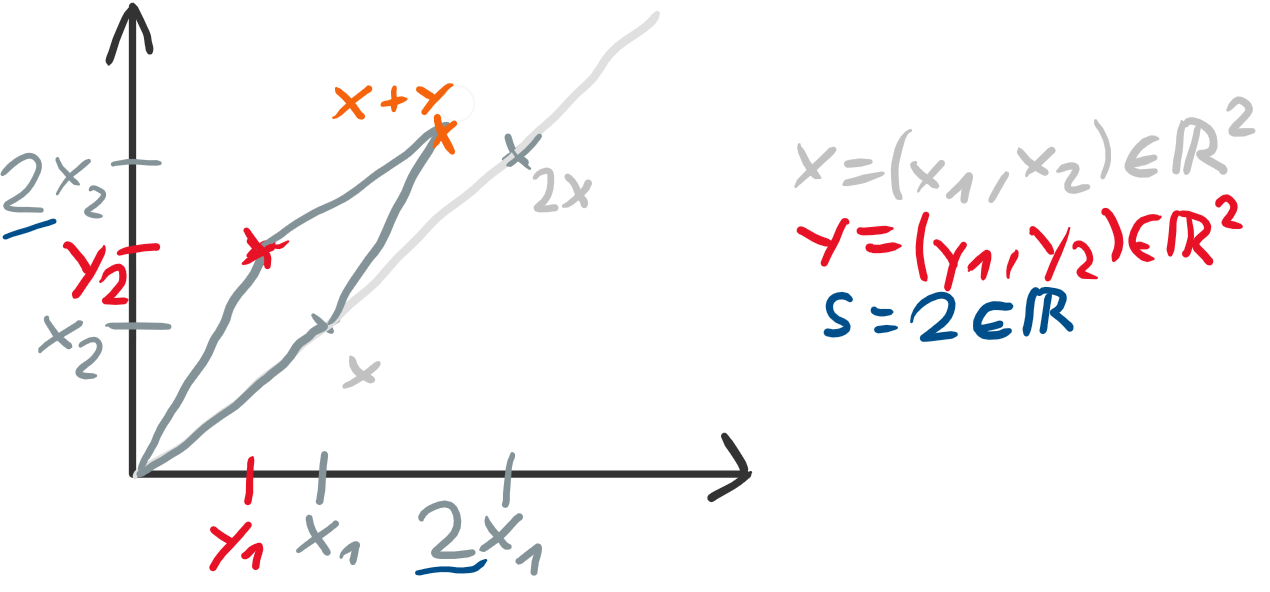
\includegraphics[width=0.7\linewidth]{img/def7-1bsp}
						\end{center}
					\end{itemize}
				
					\begin{enumerate}
						\item[b)] $(\mathbb{C}, +, \cdot)$ ist $\mathbb{C}$-VR, $\mathbb{R}$-VR, $\mathbb{Q}$-VR.
						\item[c)] Sei $M \neq \emptyset$ eine Menge, $(K, +, \cdot)$ ein Körper. Sei $V:= \{f:M \to K\}$. Betrachte
							\begin{align}
								(f \circleplus g)(x) &:= f(x) + g(x)\\
								(s \circlecdot f)(x) &:= s \cdot (f(x))\\ \text{für }& f,g \in V, x \in M, s \in K
							\end{align}
							Dann ist $(V, \circleplus, \circlecdot)$ ein $K$-VR.
					\end{enumerate}
				
			\subsubsection{Lemma 7.2 Rechenregeln}
				Sei $(K, +, \cdot)$ ein Körper, $(V, \circleplus, \circlecdot)$ ein $K$-Vektorraum (VR). Dann gilt
				\begin{enumerate}[a)]
					\item 
						\begin{align}
							0 \cdot v &= \boldzero \text{ für alle } v \in V
						\end{align}
					\item
						\begin{align}
							s \cdot \boldzero &= \boldzero \text{ für alle } s \in K
						\end{align}
					\item Für alle $s \in K$ und $v \in V$ gilt
						\begin{align}
							s \circlecdot v = \boldzero &\Longleftrightarrow s = \boldzero \wedge v = \boldzero
						\end{align}
					\item Für alle $s \in K$ und $v \in V$ gilt
						\begin{align}
							( \underbrace{-s}_{\parbox{4em}{\footnotesize\centering inv. Elem. zu $s$ in $K$ (bzgl. $+$)}} ) \circlecdot v &= \underbrace{-(s \circlecdot v)}_{\parbox{4em}{\footnotesize\centering inv. Elem. bzgl. $\circleplus$ zu $(s\circlecdot v)$}}
						\end{align}
				\end{enumerate}
			
		\section{Unterräume}
		
			\subsubsection{Definition 7.3}
				Sei $(K, +, \cdot)$ Körper, $(V, \circleplus, \circlecdot)$ ein $K$-VR. Dann heißt $U \subseteq V$ \emph{Unter(vektor)raum oder Teilraum}\subkeywordNoprint{Unter(vektor)raum}{Vektorräume}\subkeywordNoprintUnwichtig{Teilraum}{Vektorräume} von $V$, falls gilt
				\begin{enumerate}
					\item $U \neq \emptyset$
					\item $v,w \in U \implies v \circleplus w \in U$
					\item $s \in K, v \in U \implies s \circlecdot v \in U$
				\end{enumerate}
				\paragraph{Bemerkung}\abbrev{UVR}{Unter(vektor)raum} Ist $U\subseteq V$ ein Untervektorraum (UVR) dann ist $(U, \circleplus, \circlecdot)$ ein $K$"~VR.
				\paragraph{Beispiele}
					\begin{enumerate}[a)]
						\item $V, \{\boldzero\}$ sind UVR.
						\item Sei $v \in V \backslash \{\boldzero\}$. Dann ist $\{ v \}$ kein UVR, denn $0 \circlecdot v = \boldzero \notin \{ v \}$.
						\item Für $v \in V$ ist
							\begin{align}
								\langle v \rangle := \{s\circlecdot v: s \in K \}
							\end{align}
							ein UVR.
					\end{enumerate}
					%TODO Grafik
					
					
					
		\section{Erzeugendensysteme}
			
				\subsubsection{Definition 7.4}
					
					\begin{enumerate}[a)]
						\item Sei $(V, \circleplus, \circleplus)$ ein $K$-VR, $v_1,\dots,v_n \in V$. Dann heißt $V \in V$ \subkeyword{Linearkombination}{Vektorräume} von $v_1,\dots , v_n$, falls es $s_1,\dots , s_n$ gibt mit
						\begin{align}
							v &= (s_1 \circlecdot v_1) \circleplus (s_2 \circlecdot v_2) \circleplus \dots \circleplus (s_n \circlecdot v_n)
						\end{align}
						\item Ist $M \subseteq V$ mit $M \neq \emptyset$, so definieren wir das \subkeyword{Erzeugnis}{Vektorräume} von $M$ als
						\begin{align}
							\langle M \rangle &:= \{v \in V: v \text{ ist Linearkombination von endlich vielen Vektoren von } M\}\\
								&=: \romanspan(M)
						\end{align}
						Wir definieren:
						\begin{align}
							\langle \emptyset \rangle &:= \{ \boldzero \}
						\end{align}
					\end{enumerate}
				
					\paragraph{Bemerkung} Der $K$-VR $(K, +, \cdot)$ hat nur die Un\-ter\-vek\-tor\-räu\-me $K$ und $ \{ \underbrace{0}_{=\boldzero} \}$.
					
					%TODO viellecht ein paar Beispiele
					
				\subsubsection{Lemma 7.5}
					Sei $(V, \circleplus, \circlecdot)$ ein $K$-VR, $M\subseteq V$ beliebige Teilmenge. Dann ist $\langle M \rangle$ ein UVR von $V$.
				
					
		\section{Lineare Unabhängigkeit}
			
				\subsubsection{Definition 7.6}
					
					Sei $(V, \circleplus, \circlecdot)$ ein $K$-VR.
					
					\begin{enumerate}[a)]
						\item Vektoren $v_1, \dots, v_n$ heißen \subkeyword{linear unabhängig}{Vektorräume}, falls folgendes gilt:
						\begin{align}
							\lincombine{s}{v}{1}{n} = \boldzero \text{ mit } s_1, \dots, s_n \in K \implies s_1 = \dots = s_n = 0
						\end{align}
						Andernfalls heißen $v_1, \dots, v_n$ \subkeyword{linear abhängig}{Vektorräume}.
						\item Eine Teilemenge $M \subseteq V, M \neq \emptyset$ heißt \subkeyword{linear unabhängig}{Vektorräume}, falls je endlich viele paarweise verschiedene Vektoren aus $M$ linear unabhängig sind. Wir definieren $\emptyset$ als linear unabhängig. Ist $M \subseteq V$ nicht linear unabhängig, so heißt $M$ \subkeyword{linear abhängig}{Vektorräume}.
					\end{enumerate}
				
				\paragraph{Bemerkung}
					\begin{itemize}
						\item Jede Menge, die eine linear abhängige Teilmenge enthält ist linear abhängig.
						\item Jede Teilmenge einer linear unabhängigen Menge ist linear unabhängig.
					\end{itemize}
					
				\subsubsection{Satz 7.7}
					Sei $(V, \circleplus, \circlecdot)$ ein $K$-VR, $M \subseteq V, M \neq \emptyset, M \neq \{\boldzero\}$. Folgende Aussagen sind äquivalent:
					\begin{enumerate}
						\item $M$ ist linear abhängig.
						\item Jeder Vektor $w \in \langle M \rangle$ kann \textbf{eindeutig} geschrieben werden als Linearkombination von Vektoren aus $M$, bis auf die Reihenfolge der Summanden, d.~h.
						\begin{align}
							\text{für }& v_1, \dots, v_n \in M, s_1, \dots, s_n, t_1, \dots, t_n \in K\\
							\text{mit }& w = \lincombine{s}{v}{1}{n} = \lincombine{t}{v}{1}{n} \\
							\text{gilt }& s_1 = t_1, \dots, s_n = t_n
						\end{align}
						\item Für alle $v \in M$ gilt 
						\begin{align}
							v \notin \langle M \backslash \{ v\} \rangle
						\end{align}
						\item Für alle $v \in M$ gilt
						\begin{align}
							\langle M \backslash \{ v\} \rangle \neq \langle M \rangle
						\end{align}
					\end{enumerate}
				
				
		\section{Basis und Dimension}
		
			\subsubsection{Definition 7.8}
				Sei $V, \circleplus, \circlecdot$ $K$-VR, $M \subseteq V$.
				\begin{enumerate}[a)]
					\item $M$ heißt \subkeyword{Erzeugendensystem}{Vektorräume} von $V$, falls
						\begin{align}
							\langle M \rangle &= V
						\end{align}
					\item $M$ heißt \subkeyword{Basis}{Vektorräume} von $V$, falls $V$ ein linear unabhängiges Erzeugendensystem ist.
					\item $V$ heißt \subkeyword{endlich erzeugt}{Vektorräume}, falls $V$ ein endliches Erzeugendensystem besitzt.
				\end{enumerate}
			
				\paragraph{Beispiel}
					$\mathbb{R}^3$ als $\mathbb{R}$-VR.\\
					$\{(1,0,0),(0,1,0),(0,0,1)\}$ ist Erzeugendensystem von $\mathbb{R}^3$, denn für beliebiges $(x,y,z)\inR^3$ gilt
					\begin{align}
						(x,y,z) &= (x \circlecdot (1,0,0)) \circleplus (y\circlecdot(0,1,0)) \circleplus (z\circlecdot(0,0,1))
					\end{align}
					sogar Basis, da linear unabhängig. Insbesondere ist $\mathbb{R}^3$ endlich erzeugt.
					
				\paragraph{Bemerkung}
					Jeder VR $(K,\circleplus,\circlecdot)$ hat ein Erzeugendensystem, z.~B. $V$ selbst.
				\paragraph{Frage}
					Hat jeder endlich erzeugte VR ein Basis?
				\paragraph{Beispiel}
					$\mathbb{R}^3$ als $\mathbb{R}$-VR.
					\begin{align}
						\varepsilon = \{ (1,0,0), (0,0,0), (0,1,0), (3,4,0), (0,0,1) \} \text{ ist Erzeugendensystem von } \mathbb{R}^3
					\end{align}
					Bastele Basis $B \subseteq \varepsilon$ von $\mathbb{R}^3$: Gehe Vektoren der Reihe nach durch:
					\begin{longtable}{rl}
						$(1,0,0) \in B$, denn	& $(1,0,0) \notin \langle \emptyset \rangle = \{\boldzero\} = \{(0,0,0)\}$\\
						$(0,0,0) \notin B$, denn& $(0,0,0) \in \langle \{ (1,0,0) \} \rangle$ \\
						$(0,1,0) \in B$, denn	& $(0,1,0) \notin \langle \{ (1,0,0) \} \rangle$ \\
						$(3,4,0) \notin B$, denn& $(3,4,0) \in \langle \{ (1,0,0), (0,1,0) \} \rangle$ \\
						$(0,0,1) \in B$, denn	& $(0,0,1) \notin \langle \{ (1,0,0), (0,1,0) \} \rangle$ \\
						\multicolumn{2}{c}{$\rightarrow B = \{ (1,0,0), (0,1,0), (0,0,1) \}$}
					\end{longtable}
				
					Es gilt $B \subseteq \varepsilon$ und $B$ Basis von $\mathbb{R}^3$. Andere Basis $B' = \{(3,4,0), (1,0,0), (0,0,1)\}$.
					
			\subsubsection{Satz 7.9}
				Jeder endlich erzeugte VR besitzt eine Basis.
				\paragraph{Beweis}
					\begin{align}
						\varepsilon = \{ v_1, \dots, v_n \} \subseteq V \text{ Erzeugendensystem für } V
					\end{align}
					Bastele $B$ wie folgt:
					\begin{enumerate}
						\item Falls $v_1 \notin \langle \emptyset \rangle = \{ \boldzero \}$, dann $v_1 \in B$.\\
							Falls $v_1 \in \langle \emptyset \rangle = \{ \boldzero \}$, dann $v_1 \notin B$.
						\item Für $i = 2, \dots, n$:\\
							Falls $v_i \in \langle \{ v_1, \dots, v_i-1 \} \cap B \rangle$, dann $v_i \notin B$, andernfalls $v_i \in B$.
					\end{enumerate}
				
			\subsubsection{Satz 7.10}\label{Satz7.10}
				Sei $(V,\circleplus,\circlecdot)$ ein endlich erzeugter VR. Dann haben je zwei Basen die gleiche Anzahl an Elementen.
				\paragraph{Beweis} siehe \ref{Beweis7.10}, Seite \pageref{Beweis7.10}
				
			\subsubsection{Definition 7.11}
				Sei $(V, \circleplus, \circlecdot)$ endlich erzeugter VR. Dann heißt $V$ \emph{$n$-dimensional}\subkeywordNoprint{n-dimensional@$n$-dimensional}{Vektorräume}, $n\inN_0$, falls es ein Basis mit $n$ Elementen gibt. $n$ heißt die \subkeyword{Dimension}{Vektorräume} von $V$.
				
	\chapter{Lineare Algebra II: Lineare Abbildungen}
	
	\section{Grundlagen und Isomorphismen}
	
		\subsubsection{Definition 8.1}
			\begin{enumerate}[a)]
				\item Seinen $V, W$ $K$-VR. Eine Abbildung
					\begin{align}
						f: V \to W
					\end{align}
					heißt \emph{linear}\index{lineare Abbildungen}\index{Vektorräume!lineare Abbildungen} oder \subkeyword{Homomorphismus}{lineare Abbildungen}, falls gilt
					\begin{align}
						f(x\circleplus y) &= f(x) \circleplus f(y)\\
						f(s\circlecdot x) &= s \circlecdot f(x)\\
						\text{für alle } x,y&\in V, s \in K
					\end{align}
					Wir setzen
					\begin{align}
						L(V,W) := \{f: V \to W: f \text{ ist linear}\}
					\end{align}
				\item Eine bijektive lineare Abbildung heißt \subkeyword{Isomorphismus}{lineare Abbildungen}. Falls es einen Isomorphismus zwischen $V$ und $W$ gibt, so heißen V und W \subkeyword{isomorph}{lineare Abbildungen}.
			\end{enumerate}
		\paragraph{Notation} (ker = kernel = Kern, Im = Image = Bild)\abbrev{ker}{Kern (lineare Abbildungen)}\abbrev{Im}{Bild (lineare Abbildungen)} \subkeywordNoprint{Kern $\ker$}{lineare Abbildungen}\subkeywordNoprint{lineare Abbildungen}{Bild}\subkeywordNoprint{Bild $\romanIm$}{lineare Abbildungen}
			\begin{align}
				\text{für } & f: V \to W \text{ linear}\\
				\ker(f) &= \Kern(f) = f^{-1}(\{\boldzero_W\}) = \{v \in V : f(v) = \boldzero_W\} \subseteq V\\
				\romanIm(f) &= \{w \in W: \text{ es gibt ein } v \in V: f(v) = w \} \subseteq W
			\end{align}
			
		\subsubsection{Lemma 8.2}
			Seien $U,V,W$ $K$-VR.\\
			Sind $f: U \to V$ und $g: V \to W$ linear, dann ist auch $g \circ f: U \to W$ linear.
			
		\subsubsection{Satz 8.3}
			Seien $V,W$ $K$-VR, $\{b_1 \dots b_n\}$ Basis von $V$, $\{w_1, \dots, w_n\} \subseteq W$. Dann gibt es genau eine lineare Abbildung $f: V \to W$ mit $f(b:i) = w_i$ für alle $i \in \{1, \dots, n\}$
			
		\subsubsection{Satz 8.4}
			Seien $U, V, W$ $K$-VR.
			\begin{itemize}
				\item Ist $f: U \to V$ ein Isomorphismus\footnote{Isomorphismus = bijektive lineare Abbildung} (Iso), dann ist $f^{-1}: U \to V$ auch ein Iso.
				\item Sind $f: U \to V$ und $g: V \to W$ Iso, dann ist auch $g \circ f: U \to W$ ein Iso.
				\item Auf der Menge aller $K$-VR ist durch
					\begin{align}
						U \cong V :\Longleftrightarrow U \text{ und } V \text{ sind isomorph}
					\end{align}
					eine Äquivalenzrelation gegeben.
			\end{itemize}
		
		\subsubsection{Satz 8.5}
			Seien $U,V$ $K$-VR mit $\dim U = \dim V \inN_0$. Dann sind $U$ und $V$ isomorph.
			
			
			
		\section{Kern und Bild, Dimensionsformel}
	
			\subsubsection{Definition 8.6}
				Seien $U, V$ $K$-VR, $f : U \to V$ linear. Dann ist
				\begin{align}
					\ker(f)	&= \Kern(f) = \{u \in U: f(u) = \boldzero_V \}\\
					\romanIm(f)	&= \Bild(f) = f(U)\\
							& = \{v \in V: \text{ es gibt ein } u \in U \text{ mit } f(u) = v\}\\
							&= \{f(u):u\in U\}
				\end{align}\subkeywordNoprint{Kern $\ker$}{lineare Abbildungen}\index{ker}\index{Im}\subkeywordNoprint{lineare Abbildungen}{Bild}\subkeywordNoprint{Bild $\romanIm$}{lineare Abbildungen}
				
				\paragraph{Bemerkung} $\ker(f)$ ist UVR von $U$. $\romanIm(f)$ ist UVR von $V$.
				
			\subsubsection{Satz 8.7}
				Seien $U, V$ $K$-VR, $f: U \to V$ linear.
				\begin{enumerate}
					\item Es gilt:
						\begin{align}
							f \text{ ist injektiv} \Longleftrightarrow \ker(f) = \{\boldzero_U\}
						\end{align}
					\item Es gilt (nach Definition von Surjektivität):
						\begin{align}
							f \text{ ist surjektiv} \Longleftrightarrow \romanIm(f) = V
						\end{align}
					\item Falls $U = \langle \{u_1, \dots, u_n\} \rangle$ endlich erzeugt ist, dann ist
					\begin{align}
						\romanIm(f) = \langle \{f(u_1), \dots, f(u_n) \} \rangle
					\end{align}
				\end{enumerate}
			
			\subsubsection{Lemma 8.8}
				Sei $V$ ein endlich erzeugter $K$-VR, $V\neq \{\boldzero\}, B = \{b_1, \dots, b_n\} \subseteq V$. Folgende Aussagen sind äquivalent:
				\begin{enumerate}
					\item $B$ ist Basis von $V$.
					\item $B$ ist ein linear unabhängiges Erzeugendensystem für $V$.
					\item $B$ ist linear unabhängig und $|B| = \dim(V)$.
					\item $B$ ist linear unabhängig und $B \cup \{v\}$ ist linear abhängig für alle $v \in V \backslash B$.
					\item $B$ ist ein Erzeugendensystem für $V$, und $B \backslash \{b_i\}$ ist kein Erzeugendensystem für alle $b_i \in B$.
					\item Jedes $v\in V$ ist eine eindeutige Darstellung der Form 
					\begin{align}
						v = \lincombine{s}{b}{1}{n} \text{ mit } s_1, \dots s_n \in K
					\end{align}
					\item Ist $A = \{a_1 \dots, a_k\} \subseteq V$ linear unabhängig, dann $k \leq n$, und es gibt $(n-k)$ Elemente in $B$ so dass $A$ und diese Elemente $b_{i_1}, \dots, b_{i_{n-k}}$ eine Basis von $V$ bilden.
				\end{enumerate}
			
			\subsubsection{Satz 8.9}
				Seien $U,V$ $K$-VR, $\dim(U) = n \inN_0$. Sei $f: U \to V$ linear. Dann gilt
					\begin{align}
						\dim(U) = \dim(\ker(f)) + \dim(\romanIm(f))
					\end{align}
				
			\subsubsection{Korollar 8.10}
				Seien $U,V$ $K$-VR mit $\dim(U) = \dim(V) \inN_0, f: U \to V$ linear. Dann gilt
				\begin{align}
					f \text{ injektiv} \Longleftrightarrow f \text{ surjektiv} \Longleftrightarrow f \text{ bijektiv}
				\end{align}
			
		\section{Matrizen}
			
			\subsubsection{Idee}
				$U,V$ $K$-VR, $f: U\to V$ linear, $U$ endlich erzeugt.\\
				$f$ ist eindeutig bestimmt durch die Bilder einer Basis von $U$.\\
				$B = \{b_1, \dots, b_n\}$ Basis von $U$\\
				\begin{align}
					\begin{bmatrix}
						f(b_1)	& \cdots	& f(b_n)
					\end{bmatrix}
				\end{align}
				
			\subsubsection{Notation}
			
				Von jetzt an schreiben wir Vektoren von $K^n$ ``vertikal'', also\\
				\begin{align}
					K^n &= \left\{ \begin{pmatrix}
						x_1 \\ x_2 \\ \vdots \\ x_n
					\end{pmatrix} : x_i \in K, i = 1, \dots, n \right\} \text{ mit} \\
					\begin{pmatrix}
						x_1 \\ \vdots \\ x_n
					\end{pmatrix} \circleplus
					\begin{pmatrix}
						y_1 \\ \vdots \\ y_n
					\end{pmatrix} &= \begin{pmatrix}
						x_1 + y_1 \\ \vdots \\ x_n + y_n
					\end{pmatrix}\\
						s \circlecdot \begin{pmatrix}
						x_1 \\ \vdots \\ x_n
					\end{pmatrix} &= \begin{pmatrix}
						s \cdot x_1 \\ \vdots \\ s \cdot x_n
					\end{pmatrix}, \text{ für } x_1, \dots, x_n, y_1, \dots, y_n, s \in K
				\end{align}
			
			\subsubsection{Definition 8.11}
				Sei $(K, +, \cdot)$ ein Körper, $m, n \inN$. Eine \emph{$(m \times n)$-Matrix mit Einträgen aus $K$}\subkeywordNoprint{Matrix mit Einträgen aus K@$(m \times n)$-Matrix mit Einträgen aus $K$}{Matrizen} ist ein rechteckiges Schema
				\begin{align}
					\begin{bmatrix}
						a_{11}	& \cdots	& a_{1n}\\
						\vdots	& \ddots	& \vdots\\
						a_{m1}	& \cdots	& a_{mn}
					\end{bmatrix}
				\end{align}
				aus $m$ Zeilen und $n$ Spalten mit Einträgen $a_{ij} \in K, 1 \leq i \leq m, 1 \leq j \leq n$.\\
				$i \in \{ 1, \dots, m \}$ ist Zeilenindex, $j \in \{1, \dots, n \}$ ist Spaltenindex.\\
				Schreibweise: $(a_{ij})$ oder $\matrixwithsubscript{a}{i}{j}{m}{n}$\\
				Die Menge aller $(m \times n)$-Matrizen mit Einträgen aus $K$ bezeichnen wir mit $K^(m \times n)$.
				
				\paragraph{Bemerkung} Wir identifizieren $K^n \entspricht K^{n \times 1}$
				
			\subsubsection{Definition 8.12}
				Seien $U, V$ zwei $K$-VR, $B = \{b_1, \dots, b_n\} \subseteq U$ Basis von $U$, $P = \{p_1, \dots, p_m\} \subseteq V$ Basis von V. Sei $f: U \to V$ linear. Für $j = 1, \dots, n$
				\begin{align}
					&f(b_j) = (a_{1j} \circlecdot p_1) \circleplus \dots \circleplus (a_{mj} \circlecdot p_m)\\
					&\text{ mit } a_{ij} \in K \text{ für alle } i \in \{1, \dots, m\}, j \in \{1, \dots, n\}
				\end{align}
				Dann heißt $\matrixwithsubscript{a}{i}{j}{m}{n}$ die \subkeyword{Darstellungsmatrix}{Matrizen} von $f$ bezüglich der Basen $B$ und $P$.
				
				\paragraph{Bemerkung} ``In der Darstellungsmatrix stehen in den Spalten die Basen der Basisvektoren.''
				
				\paragraph{Beispiele}
					Sei $f: \mathbb{R}^2 \to \mathbb{R}^3, f\left(\begin{pmatrix}
						x \\ y
					\end{pmatrix}\right) = \begin{pmatrix}
					x+y \\ -y \\ x-y
					\end{pmatrix}$
					\begin{itemize}
						\item Betrachte Standardbasen $B = \left\{ \begin{pmatrix} 1 \\ 0 \end{pmatrix}, \begin{pmatrix} 0 \\ 1 \end{pmatrix} \right\} \subset \mathbb{R}^2,\\
						P = \left\{ \begin{pmatrix} 1 \\ 0 \\ 0 \end{pmatrix}, \begin{pmatrix} 0 \\ 1 \\ 0 \end{pmatrix}, \begin{pmatrix} 0 \\ 0 \\ 1 \end{pmatrix} \right\} \subset \mathbb{R}^3$\\
						Dann
						\begin{align}
							f\left( \begin{pmatrix}
								1 \\ 0
							\end{pmatrix}  \right) &= \begin{pmatrix}
								1 \\ 0 \\ 1
							\end{pmatrix} = 1 \circlecdot \begin{pmatrix}
								1 \\ 0 \\ 0
							\end{pmatrix} \circleplus 0 \circlecdot \begin{pmatrix}
								0 \\ 1 \\ 0
							\end{pmatrix} \circleplus 1 \circlecdot \begin{pmatrix}
								0 \\ 0 \\ 1
							\end{pmatrix}\\
							f\left( \begin{pmatrix}
							0 \\ 1
							\end{pmatrix}  \right) &= \begin{pmatrix}
							1 \\ -1 \\ -1
							\end{pmatrix} = 1 \circlecdot \begin{pmatrix}
							1 \\ 0 \\ 0
							\end{pmatrix} \circleplus (-1) \circlecdot \begin{pmatrix}
							0 \\ 1 \\ 0
							\end{pmatrix} \circleplus (-1) \circlecdot \begin{pmatrix}
							0 \\ 0 \\ 1
							\end{pmatrix}\\
							\rightarrow& \text{ Darstellungsmatrix }\begin{bmatrix}
							1	& 1 \\
							0	& -1 \\
							1	& -1
							\end{bmatrix} \in \mathbb{R}^{3 \times 2}
						\end{align}
						
						\item Betrachte $B = \left\{ \begin{pmatrix} 1 \\ 1 \end{pmatrix}, \begin{pmatrix} 1 \\ -1 \end{pmatrix} \right\} \subset \mathbb{R}^2, P = \left\{ \begin{pmatrix} 1 \\ 0 \\ 0 \end{pmatrix}, \begin{pmatrix} 0 \\ 1 \\ 0 \end{pmatrix}, \begin{pmatrix} 0 \\ 0 \\ 1 \end{pmatrix} \right\} \subset \mathbb{R}^3$\\
						Es gilt
						\begin{align}
							f\left( \begin{pmatrix}
							1 \\ 1
							\end{pmatrix}  \right) &= \begin{pmatrix}
							2 \\ -1 \\ 0
							\end{pmatrix} = 2 \circlecdot \begin{pmatrix}
							1 \\ 0 \\ 0
							\end{pmatrix} \circleplus (-1) \circlecdot \begin{pmatrix}
							0 \\ 1 \\ 0
							\end{pmatrix} \circleplus 0 \circlecdot \begin{pmatrix}
							0 \\ 0 \\ 1
							\end{pmatrix}\\
							f\left( \begin{pmatrix}
							1 \\ -1
							\end{pmatrix}  \right) &= \begin{pmatrix}
							0 \\ 1 \\ 2
							\end{pmatrix} = 0 \circlecdot \begin{pmatrix}
							1 \\ 0 \\ 0
							\end{pmatrix} \circleplus 1 \circlecdot \begin{pmatrix}
							0 \\ 1 \\ 0
							\end{pmatrix} \circleplus 2 \circlecdot \begin{pmatrix}
							0 \\ 0 \\ 1
							\end{pmatrix}\\
							\rightarrow& \text{ Darstellungsmatrix }\begin{bmatrix}
							2	& 0 \\
							-1	& 1 \\
							0	& 2
							\end{bmatrix} \in \mathbb{R}^{3 \times 2}
						\end{align}
						
						\item Betrachte $B = \left\{ \begin{pmatrix} 1 \\ 0 \end{pmatrix}, \begin{pmatrix} 0 \\ 1 \end{pmatrix} \right\} \subset \mathbb{R}^2, P = \left\{ \begin{pmatrix} 1 \\ 0 \\ 0 \end{pmatrix}, \begin{pmatrix} 1 \\ 1 \\ 0 \end{pmatrix}, \begin{pmatrix} 1 \\ 1 \\ 1 \end{pmatrix} \right\} \subset \mathbb{R}^3$\\
						Es gilt
						\begin{align}
							f\left( \begin{pmatrix}
							1 \\ 0
							\end{pmatrix}  \right) &= \begin{pmatrix}
							1 \\ 0 \\ 1
							\end{pmatrix} = 1 \circlecdot \begin{pmatrix}
							1 \\ 0 \\ 0
							\end{pmatrix} \circleplus (-1) \circlecdot \begin{pmatrix}
							1 \\ 1 \\ 0
							\end{pmatrix} \circleplus 1 \circlecdot \begin{pmatrix}
							1 \\ 1 \\ 1
							\end{pmatrix}\\
							f\left( \begin{pmatrix}
							0 \\ 1
							\end{pmatrix}  \right) &= \begin{pmatrix}
							1 \\ -1 \\ -1
							\end{pmatrix} = 2 \circlecdot \begin{pmatrix}
							1 \\ 0 \\ 0
							\end{pmatrix} \circleplus 0 \circlecdot \begin{pmatrix}
							1 \\ 1 \\ 0
							\end{pmatrix} \circleplus (-1) \circlecdot \begin{pmatrix}
							1 \\ 1 \\ 1
							\end{pmatrix}\\
							\rightarrow& \text{ Darstellungsmatrix }\begin{bmatrix}
							1	& 2 \\
							-1	& 0 \\
							0	& -1
							\end{bmatrix} \in \mathbb{R}^{3 \times 2}
						\end{align}
					\end{itemize}
				
				\paragraph{Beobachtung}
					Sei $f: K^n \to K^m$ linear mit Darstellungsmatrix $A = \matrixwithsubscript{a}{i}{j}{m}{n}$ bzgl. Standardbasen. Dann gilt für $x = \begin{pmatrix}
						x_1 \\ \vdots \\ x_n
					\end{pmatrix} \in K^n$
					\begin{align}
						f(x) &= f\left( x_1 \circlecdot \begin{pmatrix}
							1 \\ 0 \\ \vdots \\ 0
						\end{pmatrix} \circleplus \dots \circleplus x_n \circlecdot \begin{pmatrix}
							0 \\ \vdots \\ 0 \\ 1
						\end{pmatrix} \right) \\
						&\overset{f\text{ linear}}{=} x_1 \cdot f\left( \begin{pmatrix}
							1 \\ 0 \\ \vdots \\ 0
						\end{pmatrix} \right)\circleplus \dots \circleplus x_n \circlecdot f\left( \begin{pmatrix}
							0 \\ \vdots \\ 0  \\ 1
						\end{pmatrix} \right) \\
						&= x_1 \circlecdot \begin{pmatrix}
							a_{11} \\ \vdots \\ a_{m1}
						\end{pmatrix} \circleplus \dots \circleplus x_n \circlecdot \begin{pmatrix}
							a_{1n} \\ \vdots \\ a_{mn}
						\end{pmatrix}
					\end{align}
					
			\subsubsection{Definition 8.13}
				Wir definieren für ${\color{gray} (a_{ij}) =\ } A \in K^{m \times n}$ und ${\color{gray} \begin{pmatrix}
						x_1 \\ \vdots \\ x_n
					\end{pmatrix} =\ } x \in K^n$
				
					\begin{align}
						A \cdot x &= \begin{bmatrix}
							a_{11}	& \cdots	& a_{1n} \\
							\vdots	& \ddots	& \vdots \\
							a_{m1}	& \cdots	& a_{mn}
						\end{bmatrix} \cdot \begin{bmatrix}
							x_1 \\ \vdots \\ x_n
						\end{bmatrix} = \begin{bmatrix}
							a_{11} \cdot x_1 + \cdots + a_{1n} \cdot x_n \\
							\vdots \\
							a_{m1} \cdot x_1 + \cdots + a_{mn} \cdot x_n
						\end{bmatrix}
					\end{align}
			
			\subsubsection{Satz 8.14}
				\begin{enumerate}[a)]
					\item Sei $B \in K^{m \times n}$. Dann ist die Abbildung $g: K^n \to K^m, g(x) := B \cdot x$ linear.
					\item Sei $f: K^n \to K^m$ linear. Dann gibt es eine Matrix $A \in K^{m \times n}$ so dass $f(x) = A \cdot x$ für alle $x \in K^n$.
				\end{enumerate}
			
			\subsubsection{Definition 8.15}
				\begin{enumerate}[a)]
					\item Für $A \in K^{m \times n}, B \in K^{l \times m}$ definieren wir $BA \in K^{k \times n}$ als
					\begin{align}
						(B\cdot A)_{rs} &= \sum_{i = 1}^{m} b_{ri} \cdot a_{is}, r \in \{1,\dots,l\}, s \in \{1,\dots, n \}
					\end{align}
					\begin{center}
						\textit{``Zeile mal Spalte''}
					\end{center}
					\item Für $A, A' \in K^{m\times n}$ definieren wir $A + A' \in K^{m\times n}$ als
					\begin{align}
						(A+A')_{ij} &= a_{ij} + a'_{ij}
					\end{align}
				\end{enumerate}
			
				\paragraph{Bemerkung}~\\
					\begin{tabular}{llll}
						Falls & $A$ & Darstellungsmatrix zu & $f: K^n \to K^m$ \\
							& $A'$ & Darstellungsmatrix zu & $f': K^n \to K^m$ \\
							& $B$ & Darstellungsmatrix zu & $g: K^m \to K'$ \vspace{0.5em}\\
						dann & $(A+A')$ & Darstellungsmatrix zu & $f+f': K^n \to K^m$ \\ 
							& $B\times A$ & Darstellungsmatrix zu & $g\circ f: K^n \to K'$
					\end{tabular} %TODO Verfifizieren, ob das so richtig ist
		
				
					
			
	%\iffalse
	\appendix
		
	\chapter{Beweise}
		
		\iffalse
		
		\section{zu Kapitel 2 Relationen \& Funktionen}
		
			\subsubsection{Beweis zu Satz 2.11}\label{Beweis2.11}
			
			\shadowbox{
				\begin{minipage}[h]{\linewidth}
					\textbf{Satz 2.11}\\
					Sei $f: X \rightarrow Y$ eine Abbildung. Die folgenden Aussagen sind äquivalent:
					\begin{align}
					(A) &\ f \text{ ist bijektiv}\\
					(B) &\ \text{Es gibt eine Abbildung }g: Y \rightarrow X\text{, so dass }g=f=\id_X\text{ und }f=g=\id_Y \label{eq:2.11B}
					\end{align}
				\end{minipage}
			}
			%TODO Beweis aufschreiben
		\fi	
			
		\section{zu Kapitel 8 Lineare Algebra II: Lineare Abbildungen}
		
			\subsubsection{Beweis Satz 7.10}\label{Beweis7.10}
			
			\shadowbox{
				\begin{minipage}[h]{\linewidth}
					\textbf{Satz 7.10} (\ref{Satz7.10}, Seite \pageref{Satz7.10})\\
					Sei $(V,\circleplus,\circlecdot)$ ein endlich erzeugter VR. Dann haben je zwei Basen die gleiche Anzahl an Elementen.
				\end{minipage}
			}
			Idee des Beweises: ``Basisaustausch''.
			\paragraph{Beispiel}
				$\mathbb{R}^2$ als $\mathbb{R}$-VR, $B = \{(1,0),(0,1)\}$ Basis.\\
				Betrachte $A = \{(1,1),(5,3),(3,5)\}$. Beobachtung: $A \nsubseteq \langle \{(1,0) \} \rangle$\\
				Wir haben z.~B.
				\begin{align}
					&\underbrace{(1,1)}_{\in A} = (1,0) \circleplus (0,1)\\
					\implies& (0,1) = (1,1) \circleplus [(-1) \circlecdot (0,1)]\\
					\implies& \{(1,1),(0,1)\} \text{ ist Erzeugendensystem von } \mathbb{R}^2
				\end{align}
				Nächster Schritt: Es gilt
				\begin{align}
					&(5,3) = (5 \circlecdot (1,1)) \circleplus ((-2) \circlecdot (0,1)) \implies (0,1) \in \langle \{(5,3),(1,1)\} \rangle\\
					\implies & \{(5,3),(1,1)\} \text{ ist Erzeugendensystem von } \mathbb{R}^2\\
					\implies & (3,5) \in \langle \{ (5,3), (1,1) \} \implies A \text{ ist linear abhängig}
				\end{align}
				
			\paragraph{Beweis} des Satzes: Wir zeigen: Falls $\{b_1,\dots,b_n\}, n \inN_0$ ein Erzeugendensystem von $V$ ist und $A = \{ a_1, \dots a_{n+1}\}, |A| = n+1$, dann ist $A$ linear abhängig, also insbesondere keine Basis.\\
			Vollständige Induktion nach $n$:
			\pagebreak[3]
			\begin{itemize}\nopagebreak[4]
				\item[I.~A.:] \nopagebreak[4]$n=0$\nopagebreak[4]\\ \nopagebreak[4]
					\nopagebreak[4]\begin{align}
						V = \langle \emptyset \rangle = \{\boldzero\} & \implies A = \{\boldzero\} \text{ (einzige Teilmenge von } V \text{ mit einem Element)}\\
						& \implies A \text{ linear abhängig}
					\end{align}
				\item[I.~V.:] Falls $\tilde{V} \subseteq V$ von $k$ Vektoren aus $V$ erzeugt wird mit $k \leq n \inN_0$ beliebig, aber fest, dann ist je $(k+1)$ Vektoren aus $\tilde{V}$ linear abhängig.
				\item[I.~S.:] Sei $\tilde{V} = \langle \{ b_1, \dots, b_{n+1} \} \rangle, A = \{ a_1, \dots, a_{n+2} \}, |A| = n+2$
			\end{itemize}
		Angenommen $A$ ist linear unabhängig.\\
		Zwei Möglichkeiten:
		\begin{enumerate}
			\item $\underbrace{A}_\text{2 Vektoren} \subseteq \lbrace \{ b_2, \dots, b_{n+1} \} \rbrace \implies$ nach I.~V. ist $A$ linear unabhängig. \lightning
			\item Es gibt ein $a \in A$, o.~E.\footnote{ohne Einschränkung} $a_1$ (umnummerieren möglich), so dass
			\begin{align}
				a_1 \in \langle \{b_2, \dots, b_{n+1}\} \rangle
			\end{align}
			$\implies$ Jede Linearkombination $a_1 =  \lincombine{s}{b}{1}{n+1}, s_i \in K$ erfüllt $s_1 \neq 0$
			\begin{align}
				&\implies b_1 = s_1^{-1} \cdot a_1 - s_1^{-1} \cdot [\lincombine{s}{b}{2}{n+1}]
				&\implies \{a_1, b_2, \dots, b_{n+1}\} \text{ ist Erzeugendensystem von } V
			\end{align}
			Falls $\underbrace{\{a_2, \dots, a_{n+1}\}}_{n+1\text{ Vektoren}} \subseteq \langle \underbrace{\{\cancel{a_1}, b_3, \dots b_{n+1}\}}_{\cancelto{n-1}{n} \text{ Vektoren}}$, dann sind $a_2, \dots a_{n+2}$ linear abhängig. \lightning\\
			Ähnlich wie oben: o.~E.
			\begin{align}
				\{a_1, a_2, b_3, \dots, b_{n+1}\} \text{ Erzeugendensystem}
			\end{align}
			Rest: Übungsblatt
		\end{enumerate}
		
		
		
		
		
			
	%\fi
	\printindex
\end{document}